% Options for packages loaded elsewhere
\PassOptionsToPackage{unicode}{hyperref}
\PassOptionsToPackage{hyphens}{url}
%
\documentclass[
  11pt,
]{article}
        \usepackage{amsmath,amssymb}
        \usepackage{lmodern}
            \usepackage{iftex}
    \ifPDFTeX
      \usepackage[T1]{fontenc}
      \usepackage[utf8]{inputenc}
      \usepackage{textcomp} % provide euro and other symbols
    \else % if luatex or xetex
          \usepackage{unicode-math}
          \defaultfontfeatures{Scale=MatchLowercase}
      \defaultfontfeatures[\rmfamily]{Ligatures=TeX,Scale=1}
                                    \fi
            % Use upquote if available, for straight quotes in verbatim environments
    \IfFileExists{upquote.sty}{\usepackage{upquote}}{}
    \IfFileExists{microtype.sty}{% use microtype if available
      \usepackage[]{microtype}
      \UseMicrotypeSet[protrusion]{basicmath} % disable protrusion for tt fonts
    }{}
        \makeatletter
    \@ifundefined{KOMAClassName}{% if non-KOMA class
      \IfFileExists{parskip.sty}{%
        \usepackage{parskip}
      }{% else
        \setlength{\parindent}{0pt}
        \setlength{\parskip}{6pt plus 2pt minus 1pt}}
}{% if KOMA class
  \KOMAoptions{parskip=half}}
\makeatother
\usepackage{xcolor}
\usepackage[margin=1.2in]{geometry}
\usepackage{longtable,booktabs,array}
\usepackage{calc} % for calculating minipage widths
% Correct order of tables after \paragraph or \subparagraph
\usepackage{etoolbox}
\makeatletter
\patchcmd\longtable{\par}{\if@noskipsec\mbox{}\fi\par}{}{}
\makeatother
% Allow footnotes in longtable head/foot
\IfFileExists{footnotehyper.sty}{\usepackage{footnotehyper}}{\usepackage{footnote}}
\makesavenoteenv{longtable}
\usepackage{graphicx}
\makeatletter
\def\maxwidth{\ifdim\Gin@nat@width>\linewidth\linewidth\else\Gin@nat@width\fi}
\def\maxheight{\ifdim\Gin@nat@height>\textheight\textheight\else\Gin@nat@height\fi}
\makeatother
% Scale images if necessary, so that they will not overflow the page
% margins by default, and it is still possible to overwrite the defaults
% using explicit options in \includegraphics[width, height, ...]{}
\setkeys{Gin}{width=\maxwidth,height=\maxheight,keepaspectratio}
% Set default figure placement to htbp
\makeatletter
\def\fps@figure{htbp}
\makeatother
\setlength{\emergencystretch}{3em} % prevent overfull lines
\providecommand{\tightlist}{%
  \setlength{\itemsep}{0pt}\setlength{\parskip}{0pt}}
\setcounter{secnumdepth}{5}
\newlength{\cslhangindent}
\setlength{\cslhangindent}{1.5em}
\newlength{\csllabelwidth}
\setlength{\csllabelwidth}{3em}
\newlength{\cslentryspacingunit} % times entry-spacing
\setlength{\cslentryspacingunit}{\parskip}
\newenvironment{CSLReferences}[2] % #1 hanging-ident, #2 entry spacing
 {% don't indent paragraphs
  \setlength{\parindent}{0pt}
  % turn on hanging indent if param 1 is 1
  \ifodd #1
  \let\oldpar\par
  \def\par{\hangindent=\cslhangindent\oldpar}
  \fi
  % set entry spacing
  \setlength{\parskip}{#2\cslentryspacingunit}
 }%
 {}
\usepackage{calc}
\newcommand{\CSLBlock}[1]{#1\hfill\break}
\newcommand{\CSLLeftMargin}[1]{\parbox[t]{\csllabelwidth}{#1}}
\newcommand{\CSLRightInline}[1]{\parbox[t]{\linewidth - \csllabelwidth}{#1}\break}
\newcommand{\CSLIndent}[1]{\hspace{\cslhangindent}#1}
\DeclareMathSymbol{\shortminus}{\mathbin}{AMSa}{"39}
\newcommand{\Ex}{\mathbb{E}}
\newcommand{\Var}{\mathrm{Var}}
\newcommand{\HW}{\mathrm{HW}}
\newcommand{\RI}{\mathrm{RI}}
\newcommand{\Bin}{\mathrm{Binomial}}
\newcommand{\Uniform}{\mathrm{Uniform}}
\newcommand{\Beta}{\mathrm{Beta}}
\newcommand{\Exp}{\mathrm{Exponential}}
\newcommand{\Gam}{\mathrm{Gamma}}
\newcommand{\Bfun}{\mathrm{B}}
\newcommand{\eps}{\epsilon}
\newcommand{\all}{A}
\newcommand{\erf}{\mathrm{erf}}
\newcommand{\erfi}{\mathrm{erfi}}
\newcommand{\fix}{\mathrm{fix}}
\newcommand{\logit}{\mathop{\mathrm{logit}}}
\usepackage{caption}
\captionsetup[figure]{labelfont=bf,font=small}
\usepackage{float,soul}
\usepackage[normalem]{ulem}
\makeatletter
\def\fps@figure{tb}
\makeatother
\usepackage{algorithm}
\usepackage{algpseudocode}
\usepackage{lipsum}
\makeatletter
\@ifpackageloaded{subfig}{}{\usepackage{subfig}}
\@ifpackageloaded{caption}{}{\usepackage{caption}}
\captionsetup[subfloat]{margin=0.5em}
\AtBeginDocument{%
\renewcommand*\figurename{Figure}
\renewcommand*\tablename{Table}
}
\AtBeginDocument{%
\renewcommand*\listfigurename{List of Figures}
\renewcommand*\listtablename{List of Tables}
}
\newcounter{pandoccrossref@subfigures@footnote@counter}
\newenvironment{pandoccrossrefsubfigures}{%
\setcounter{pandoccrossref@subfigures@footnote@counter}{0}
\begin{figure}\centering%
\gdef\global@pandoccrossref@subfigures@footnotes{}%
\DeclareRobustCommand{\footnote}[1]{\footnotemark%
\stepcounter{pandoccrossref@subfigures@footnote@counter}%
\ifx\global@pandoccrossref@subfigures@footnotes\empty%
\gdef\global@pandoccrossref@subfigures@footnotes{{##1}}%
\else%
\g@addto@macro\global@pandoccrossref@subfigures@footnotes{, {##1}}%
\fi}}%
{\end{figure}%
\addtocounter{footnote}{-\value{pandoccrossref@subfigures@footnote@counter}}
\@for\f:=\global@pandoccrossref@subfigures@footnotes\do{\stepcounter{footnote}\footnotetext{\f}}%
\gdef\global@pandoccrossref@subfigures@footnotes{}}
\@ifpackageloaded{float}{}{\usepackage{float}}
\floatstyle{ruled}
\@ifundefined{c@chapter}{\newfloat{codelisting}{h}{lop}}{\newfloat{codelisting}{h}{lop}[chapter]}
\floatname{codelisting}{Listing}
\newcommand*\listoflistings{\listof{codelisting}{List of Listings}}
\makeatother
\ifLuaTeX
  \usepackage{selnolig}  % disable illegal ligatures
\fi
\IfFileExists{bookmark.sty}{\usepackage{bookmark}}{\usepackage{hyperref}}
\IfFileExists{xurl.sty}{\usepackage{xurl}}{} % add URL line breaks if available
\urlstyle{same} % disable monospaced font for URLs
\hypersetup{
  pdftitle={Polygenic barriers to gene flow: the role of dominance, haploid selection and heterogeneous genetic architectures},
  pdfkeywords={local adaptation, reproductive isolation, haplodiplontic
life cycle, dominance, linkage disequilibrium, genetic drift,
distribution of fitness effects, mainland-island model},
  hidelinks,
  pdfcreator={LaTeX via pandoc}}


\title{Polygenic barriers to gene flow: the role of dominance, haploid
selection and heterogeneous genetic architectures}
\author{
Arthur Zwaenepoel\(^{1,\ast}\), Himani
Sachdeva\(^{2,\ddagger}\),Christelle Fraïsse\(^{1,\ddagger}\)
\textsuperscript{}
}
\date{\footnotesize{ 1. University of Lille, CNRS, UMR 8198 --
Evo-Eco-Paleo, F-59000 Lille, France \linebreak  2. Department of
Mathematics, University of Vienna, Vienna,
Austria \linebreak  \(^\ast\)\texttt{arthur.zwaenepoel@univ-lille.fr},
\(^\ddagger\)contributed equally \linebreak }}


\begin{document}
\maketitle
\begin{abstract}
We study the maintenance of polygenic local adaptation and its effects
on reproductive isolation in a mainland-island model for populations
with a general biphasic life cycle, encompassing haploid and diploid
models as special cases. We quantify the strength of a multilocus
barrier to gene flow due to divergent local adaptation at \(L\) unlinked
and weakly selected loci, and obtain predictions for the equilibrium
frequencies of locally adaptive alleles with arbitrary dominance and
haploid-phase selection, accounting for genetic drift using a diffusion
approximation. We extend classical single locus results on the role of
dominance in the mainland-island model to the multilocus case,
highlighting how linkage disequilibrium in multilocus barriers has
rather different effects on differentiation and swamping thresholds for
recessive alleles compared to dominant ones. Details about the biphasic
life cycle can be captured through a set of effective parameters, and we
show that for the same total strength of selection over the life cycle,
increasing the relative intensity of selection in the haploid phase
leads to stronger barriers to gene flow. We study the effect of
heterogenous genetic architectures of local adaptation on the resulting
barrier to gene flow, characterizing the realized genetic architecture
at migration-selection balance for different distributions of fitness
effects. Our results highlight the importance of barrier heterogeneity
in shaping observable patterns of differentiation between populations
under divergent selection pressures.
\end{abstract}
\small
\textbf{Keywords:} local adaptation, reproductive isolation,
haplodiplontic life cycle, dominance, linkage disequilibrium, genetic
drift, distribution of fitness effects, mainland-island model
\normalsize

\hypertarget{sec:intro}{%
\section{Introduction}\label{sec:intro}}

When a population is subdivided across multiple habitats with different
environmental conditions, the extent to which distinct subpopulations
can maintain locally beneficial genetic variation depends on the rate of
migration between them. Migration between populations that maintain
divergently selected alleles can generate migration load (a reduction in
mean fitness due to the influx of locally maladaptive genes) or may lead
to loss of local adaptation altogether (so-called \emph{swamping} by
gene flow) (e.g. Lenormand 2002). While local adaptation may be driven
by a few conspicuous loci (e.g.~adaptive melanism in peppermoths (van't
Hof \emph{et al.} 2016) or pocket mice (Nachman \emph{et al.} 2003)), it
is believed to typically be polygenic, involving alleles of different
effect at many loci across the genome (Pritchard and Di Rienzo 2010; Le
Corre and Kremer 2012; Westram \emph{et al.} 2018; Barghi \emph{et al.}
2020; Bomblies and Peichel 2022; Stankowski \emph{et al.} 2023). When
local adaptation is polygenic, migration from a population adapted to
different environmental conditions will generate linkage disequilibria
(LD) among selected loci, and the rate at which each individual invading
locally deleterious allele is eliminated will be affected by such
associations, a phenomenon often referred to as a `coupling' effect
(Barton 1983; Kruuk \emph{et al.} 1999; Feder \emph{et al.} 2012; Yeaman
2015; Sachdeva 2022). Such coupling effects will in turn affect the
equilibrium migration load and swamping thresholds for the loci under
selection. Neutral variation may also come to be associated with locally
selected alleles, so that the latter constitute a `barrier' to neutral
gene flow, increasing neutral genetic differentiation (as quantified by
\(F_{\mathrm{ST}}\) for instance) beyond the single locus neutral
expectation (Bengtsson 1985).

Barrier effects due to divergent local adaptation at many loci may play
an important role in the evolution of reproductive isolation, and hence
speciation (Nosil 2012; Barton 2020). The colonization of a new habitat
will often involve selection on polygenic traits and give rise to a
subpopulation that exhibits some divergence from its ancestors (Barton
and Etheridge 2018). Conditional on the initial succesful establishment
of such a divergent subpopulation, whether or not speciation ensues
depends on whether local adaptation can be maintained in the face of
maladaptive gene flow (if any), and on the extent to which the partial
reproductive isolation deriving from local adaptation may promote
further divergence and strengthen reproductive isolation, either through
reinforcement, coupling with intrinsic incompatibilities, or the
establishment of additional locally beneficial mutations (Barton and De
Cara 2009; Bierne \emph{et al.} 2011; Butlin and Smadja 2018; Kulmuni
\emph{et al.} 2020). In this paper, we focus on the conditions under
which polygenic local adaptation can be maintained in the face of
maladaptive gene flow, assuming local fitness to be determined by an
additive trait under directional selection.

Despite mounting evidence that local adaptation is indeed often
polygenic (Bomblies and Peichel 2022), little is known about the
underlying genetic details: How many loci are involved? What are the
typical effect sizes? Are locally beneficial alleles typically closely
linked or spread all over the genome? How non-additive is local
adaptation? \emph{etc.} (e.g. Yeaman and Whitlock 2011; Yeaman 2015;
Bomblies and Peichel 2022). Moreover, even if such details were known, a
number of open questions remain as to how the genetic architecture of
local adaptation affects the ability of a population to maintain
reproductive isolation in the face of gene flow. For instance, it is not
directly obvious whether a heterogeneous architecture comprising both
loci of small and large effect would admit more adaptive differentiation
than a homogeneous architecture with the same average selective effect
per locus. The closely related question of how much scope there is to
infer the detailed genetic architecture underlying local adaptation from
observed patterns of genomic differentiation, as for instance obtained
through so-called `genome scans', also remains largely unanswered. So
far, most theoretical models have assumed rather simple architectures,
dealing with biallelic loci with additive and equal effects on fitness
(ignoring dominance and epistasis), that are either unlinked or
uniformly spread along a block of genome (Barton 1983; Fraïsse and
Sachdeva 2021; Sachdeva 2022); and statistical approaches for the
inference of gene flow across the genome either make similarly crude
assumptions (Aeschbacher \emph{et al.} 2017), or ignore the genetic
details of local adaptation altogether (Roux \emph{et al.} 2013; Fraïsse
\emph{et al.} 2021; Laetsch \emph{et al.} 2022).

In a recent paper, Sachdeva (2022) showed that, when the loci under
selection are unlinked, the effects of LD on equilibrium differentiation
at any individual locus in a multilocus barrier can be well described by
classical (deterministic or stochastic) single locus population genetic
theory, provided that the migration rate \(m\) is substituted by an
\emph{effective} migration rate \(m_e\) (Petry 1983; Bengtsson 1985;
Barton and Bengtsson 1986; Kobayashi \emph{et al.} 2008), which captures
how gene flow at a focal locus is affected by selection against the
associated genetic background. The effective migration rate for a
neutral locus can furthermore serve as a quantitative measure of
reproductive isolation (RI), i.e.~\(\mathrm{RI}= 1-m_e/m\) (Westram
\emph{et al.} 2022). Crucially, \(m_e\) depends itself on the
frequencies of divergently selected alleles, giving rise to feedback
effects where a small increase in migration rate may cause a sudden
collapse of local adaptation (i.e.~swamping). In her paper, Sachdeva
(2022) conducted a detailed study of the joint effects of drift and LD
on swamping thresholds and neutral differentiation in the
mainland-island and infinite-island models of population subdivision,
assuming a haploid sexual life cycle and divergently selected loci of
equal effect. In this paper, we extend the theoretical framework
outlined in Sachdeva (2022), deriving an expression for the effective
migration rate for a polygenic genetic architecture with arbitrary
fitness and dominance effects across loci (referred to as a
\emph{heterogeneous} architecture or barrier) in a population with a
haplodiplontic life cycle (which includes haplontic and diplontic life
cycles as special cases). We use this \(m_e\) to build an approximation
for the marginal allele frequency distributions at migration-selection
balance in a mainland-island model, and use these tools to assess how
the effects of multilocus LD (i.e.~coupling effects) on swamping
thresholds and the genetic architecture of reproductive isolation depend
on dominance, drift, life cycle assumptions and heterogeneity in fitness
effects across loci.

\hypertarget{model-and-methods}{%
\section{Model and Methods}\label{model-and-methods}}

\hypertarget{sec:model}{%
\subsection{Haplodiplontic mainland-island model}\label{sec:model}}

Here we outline a mainland-island model for a sexual population which
may be subject to selection in both the haploid and diploid phases. We
think of this model as a caricature of a bryophyte, pteridophyte, algal
or fungal population, but as we shall see below, the model encompasses
both diplontic and haplontic life cycles as well. Throughout, we shall
assume that sexes need not be distinguished. We assume a regular and
synchronous alternation of generations, where an island population of
\(N\) haploids (gametophytes) produces an effectively infinite pool of
gametes from which \(2Nk\) gametes are sampled that unite randomly to
form \(N k\) diploid individuals (sporophytes), \(k\) being the number
of diploids per haploid individual. The diploid generation produces in
turn an effectively infinite pool of haploid spores through meiosis, of
which \(N\) are drawn to form the next haploid generation. In each
generation, we assume \(M\) haploid individuals on the island are
replaced by haploid individuals from a mainland population, where \(M\)
is Poisson distributed with mean \(Nm\). Fitness on the island is
determined by \(L\) unlinked biallelic loci which are under divergent
selection relative to the mainland. The mainland population is assumed
to have a constant, but arbitrary, genetic composition. Unless stated
otherwise, we shall assume the mainland to be fixed, at each locus, for
the locally deleterious allele on the island. Fitness effects are
allowed to vary arbitrarily across loci. Denoting the alleles at locus
\(i\) by \(A_{i,0}\) and \(A_{i,1}\), we designate by \(w_{i,j}\) the
relative fitness of the haploid genotype \(A_{i,j}\) and \(w_{i,jk}\)
the relative fitness of diploid genotype \(A_{i,j}A_{i,k}\). We suppress
the index \(i\) when considering a generic locus. We assume throughout
that \(w_0 = 1\) and \(w_1 = e^{s_1}\) for the haploid phase, and
\(w_{00} = 1, w_{01} = w_{10} = e^{s_{01}}\), and
\(w_{11} = e^{s_{11}}\) for the diploid phase. Throughout, we denote the
frequency of the allele with relative fitness \(1\) (on the island) at
locus \(i\) by \(p_i\), and the frequency of the alternative allele by
\(q_i = 1-p_i\). Fitness is determined multiplicatively across loci, so
that, for instance, the log relative fitness of a haploid individual
fixed for all the `1' alleles (genotype
\(A_{1,1},A_{2,1}, \dots, A_{L,1}\)) is given by
\(\log w = \sum_{i=1}^L s_{i,1}\). We assume that each haploid (diploid)
individual contributes gametes (spores) to the gamete (spore) pool
proportional to its fitness. We assume symmetric mutation at a small
constant rate \(u\) per locus, occurring at meiosis.

Individual-based simulations of this model are implemented in a Julia
package (Bezanson \emph{et al.} 2017) available at
\href{https://github.com/arzwa/MultilocusIsland}{\texttt{https://github.com/arzwa/MultilocusIsland}}.
In the following sections, we build up a theoretical approximation to
this fairly general multilocus model, and validate the approximations by
comparing numerical results against individual-based simulations. We
first derive the dynamics at a single locus, considering both
deterministic and stochastic models. Next, we derive an approximation to
the effective migration rate for the multilocus model using a rather
general argument based on the reproductive value of migrant individuals.
Lastly, we approximate the allele frequency dynamics of the multilocus
model by plugging in the effective migration rate, which captures the
effect of LD among selected alleles on the dynamics at a neutral locus,
in the single locus theory.

\hypertarget{single-locus-mainland-island-model}{%
\subsection{Single locus mainland-island
model}\label{single-locus-mainland-island-model}}

\hypertarget{sec:sldet}{%
\subsubsection{Deterministic dynamics}\label{sec:sldet}}

We first consider a deterministic model for the allele frequency
dynamics at a single locus, ignoring the influence of the other loci as
well as genetic drift. As shown in detail in sec.~\ref{sec:app1}, for
weak selection and migration, the dynamics of \(p\) can be described in
continuous time by the nonlinear ordinary differential equation (ODE)
\begin{equation}
   \frac{dp}{dt} = -m(p-p^\ast) -q(s_ap + s_bpq)\ ,
   \label{eq:ode}
\end{equation} where \(p^\ast\) is the frequency on the mainland of the
allele which is beneficial on the island, \(s_a = s_1 + s_{01}\) and
\(s_b = s_{11} - 2s_{01}\), the latter being a measure of dominance
(i.e.~the deviation from multiplicative fitnesses, sometimes called
\(\iota\) (Otto 2003; Manna \emph{et al.} 2011)). Usually,
\(s_1, s_{01}\) and \(s_{11}\) will be assumed to be negative, and
\(p^\ast\) will be assumed to be small, so that selection increases
\(p\), whereas migration decreases \(p\). When \(s_1 = 0\), we obtain
the standard diploid mainland-island model, which is commonly
parameterized in terms of a dominance coefficient \(h\) and selection
coefficient \(s\), so that \(s_{01} = sh\) and \(s_{11} = s\). When
\(s_1 \ne 0\) (i.e.~there is selection in the haploid phase), we can
define an effective selection coefficient \(s_e = 2s_1 + s_{11}\) and
dominance coefficient \(h_e = \frac{s_1 + s_{01}}{2s_1 + s_{11}}\)
(except when \(s_e = 0\)), so that, under weak selection, the single
locus dynamics for an arbitrary haplodiplontic life cycle can be
described by a diploid model with these effective parameters. The
equilibria of eq.~\ref{eq:ode} are analyzed in detail in
sec.~\ref{sec:mieq}.

\hypertarget{diffusion-approximation-to-the-stochastic-dynamics}{%
\subsubsection{Diffusion approximation to the stochastic
dynamics}\label{diffusion-approximation-to-the-stochastic-dynamics}}

Still considering a single locus, we now account for the effects of
drift. Denoting by \(X_n\) and \(Y_n\) the number of \(A_1\) copies in
the \(n\)th haploid, respectively diploid, generation, the life cycle as
outlined in sec.~\ref{sec:model} corresponds, for a neutral locus, to
the following Markov chain model: \begin{align}
  Y_n|X_n &\sim \mathrm{Binomial}\left(2Nk, \frac{X_n}{N}\right) \label{eq:mc1} \\
  X_{n+1}|Y_n &\sim \mathrm{Binomial}\left(N, \frac{Y_n}{2Nk}\right). \label{eq:mc2}
  \end{align} Note that one unit of time corresponds to a single
\emph{alternation} of generations, involving two sampling stages: first
we sample \(2Nk\) gametes from an infinite pool of gametes with allele
frequency \(X_n/N\) for the \(A_1\) allele (eq.~\ref{eq:mc1}), next we
sample \(N\) haploid genotypes from an infinite pool of haploid spores
where the allele is at frequency \(Y_n/2Nk\) (eq.~\ref{eq:mc2}). This
model is akin to the standard Wright-Fisher (WF) model with variable
population size, regularly alternating between \(N\) and \(2Nk\) gene
copies. The corresponding effective population size is hence
\(N_e = (N^{-1} + (2Nk)^{-1})^{-1}\), twice the harmonic mean of the
phase-specific number of gene copies (Hein \emph{et al.} 2004) (twice
because our unit of time is an alternation of generations, not a single
generation).

A similar Markov chain model can be defined for a selected locus with
migration and mutation, but we will not consider this explicitly here,
immediately considering a diffusion approximation instead. When
evolutionary forces are sufficiently weak, diffusion theory can be
applied to approximate the equilibrium allele frequency distribution
implied by such a Markov chain by a continuous density \(\phi(p)\) of
the form \begin{equation*}
  \phi(p) \propto V(p)^{-1} \exp\left[2\int_0^p \frac{M(x)}{V(x)}dx\right],
\end{equation*} (e.g. Felsenstein 2005), where for the haplodiplontic
mainland-island model, the infinitesimal mean and variance will be,
respectively, \begin{align*}
  M(p) &= -q(s_ap + s_bpq) + u(q - p) - m(p - p^\ast) \\
  V(p) &= N_e^{-1} pq\ ,
  \end{align*} where we assume mutations occur with rate \(u\) for both
alleles. This yields a probability density function for the equilibrium
allele frequency distribution \begin{equation}
  \phi(p; N_e, u, m, s) \propto p^{2N_e(u+mp^\ast)-1}q^{2N_e(u+mq^\ast)-1}e^{N_e(2s_aq + s_bq^2)},
  \label{eq:phi}
  \end{equation} where no closed form expression is known for the
normalizing constant. This is essentially Wright's distribution,
generalized to a haplodiplontic life cycle (Wright 1937).

\hypertarget{sec:ml}{%
\subsection{Multilocus model}\label{sec:ml}}

\hypertarget{effective-migration-rate}{%
\subsubsection{Effective migration
rate}\label{effective-migration-rate}}

We now derive an expression for the effective migration rate \(m_e\),
which captures the reduction in gene flow at a focal locus embedded in a
genotype with multiple selected loci due to LD. As shown formally in
Kobayashi \emph{et al.} (2008), for weak migration, the reduction in
gene flow relative to the `raw' migration rate \(m\), termed the
\emph{gene flow factor} (gff), depends on the expected reproductive
value (RV) of migrants in the resident background (i.e.~the expected
long-term contribution of a migrant individual to the neutral gene pool
on the island, relative to individuals in the resident island
population). At any time, the proportion of individuals with recent
migrant ancestry on the island is \(O(m)\), so that the probability of
individuals with migrant backgrounds mating with each other to produce,
for instance, F2 crosses of the migrant and resident genotypes, is
\(O(m^2)\), and hence negligible for sufficiently weak migration. The
descendants of a migrant individual will therefore most likely
correspond to F1 and subsequent backcross generations, so that to a good
approximation, the RV of a migrant individual depends on the relative
fitnesses of F1, BC1, BC2, \emph{etc.} individuals.

Let \(W_h^{(n)}\) and \(W_d^{(n)}\) denote the relative fitness of an
individual derived from an \(n\)th generation haploid, respectively
diploid, backcross of an initial migrant individual with the resident
population (i.e.~\(W_d^{(1)}\) is the relative fitness of an F1 diploid,
\(W_d^{(2)}\) of an offspring from a F1 \(\times\) resident cross (BC1
generation), \emph{etc.}). Assuming migration occurs in the haploid
phase before selection, the gff can be expressed as \begin{equation}
  g = \frac{m_e}{m} = \mathbb{E}\left[W_h^{(0)}\prod^\infty_{n=1}W_d^{(n)}W_h^{(n)}\right],
\end{equation} where \(W_h^{(0)}\) is the relative fitness of the
haploid migrant in the resident population (Barton and Etheridge 2018;
Sachdeva 2022; Westram \emph{et al.} 2022). Note that this involves an
expectation over all possible lines of descent of an initial migrant
spore. In practice, \(g\) is determined only by the first 10 backcross
generations or so, as subsequent backcrosses are essentially
indistinguishable from residents. In order to derive a useful
approximate expression for \(g\), we shall make two further important
assumptions: (1) both the resident and migrant gene pool, as well as
each backcross generation, is in Hardy-Weinberg and linkage equilibrium
(HWLE); (2) the expected allele frequency at any locus in any backcross
generation is midway between that of the parents (e.g.~the mean of the
mainland and island allele frequencies for the F1 generation). In
reality, due to Mendelian segregation, individuals inherit not exactly
half of the selected alleles of each parent, and this segregation
variance will lead to variation within F1s, BC1s, \emph{etc.} on which
selection can act. This will cause deviations from the midparent value
which are \(O(s^2)\), so that this last assumption becomes more
plausible when local adaptation is due to more and more loci of smaller
effect.

Under these assumptions, each of the \(W^{(n)}\) is determined solely by
the frequencies of the selected alleles in the mainland and the island
populations at the assumed equilibrium. This allows us to determine
\(\mathbb{E}[q_i^{(n)}]\), the expected frequency of the locally
deleterious allele (in the island) at locus \(i\) among \(n\)th
generation descendants from a migrant, in terms of the allele
frequencies in the mainland and island population. Indeed, assumption
(2) implies the recursive relation
\(q_{i}^{(n)} = \frac{1}{2}(q_i^{(n-1)} + q_i)\), i.e.~the average
number of selected alleles carried by an \(n\)th generation backcross is
the mean of the number of such alleles carried by an \((n-1)\)th
generation backcross and a resident individual. Hence, we have
\(\mathbb{E}[q_i^{(n)}] = \frac{1}{2^n}(q_i^\ast + (2^n - 1)\mathbb{E}[q_i])\).
Denoting the selection coefficient at locus \(i\) for the haploid phase
by \(s_{i1}\), the expected relative fitness of an \(n\)th generation
haploid descendant is \begin{align*}
\mathbb{E}\left[W_h^{(n)}\right] \approx \frac{\exp\left[\sum_{i=1}^L s_{i1}\mathbb{E}[q_i^{(n)}]\right]}
                          {\exp\left[\sum_{i=1}^L s_{i1}\mathbb{E}[q_i]\right]} 
  = \exp\left[2^{-n}\sum_{i=1}^L s_{i1}(q_i^\ast - \mathbb{E}[q_i])\right],
\end{align*} where we have assumed that per-locus selection is
sufficiently weak that \(O(s^2)\) terms can be ignored. For the diploid
phase, a similar argument shows that for the \((n+1)\)th generation,
\begin{align*}
\mathbb{E}\left[W_d^{(n+1)}\right] 
  &= \exp\left[2^{-n}\sum_{i=1}^L s_{i01}(q_i^\ast - \mathbb{E}[q_i]) 
    - s_{i,b}(p_i^\ast\mathbb{E}[q_i] - \mathbb{E}[p_iq_i])\right],
\end{align*} where \(s_{i01}\) and \(s_{i11}\) are the selection
coefficients against heterozygotes and homozygotes at locus \(i\)
respectively, and where, analogous to the single locus model,
\(s_{i,b} = s_{i11} - 2s_{i01}\). Putting everything together, the
approximate gff becomes \begin{align}
g 
 &\approx \mathbb{E}\left[W_h^{(0)}\right]\prod_{n=1}^\infty 
    \left(\mathbb{E}\left[W_d^{(n)}\right] \mathbb{E}\left[W_h^{(n)}\right]\right)
 \nonumber \\
 &=\prod_{k=0}^\infty \exp\left[ 
    2^{-k}\sum_{i=1}^L s_{i,a}(q_i^\ast - \mathbb{E}[q_i]) - 
    s_{i,b}(p_i^\ast \mathbb{E}[q_i] - \mathbb{E}[p_iq_i])\right] \nonumber \\
&=\exp\left[2\sum_{i=1}^L 
    s_{i,a}(q_i^\ast - \mathbb{E}[q_i]) - s_{i,b}(p_i^\ast\mathbb{E}[q_i] -
    \mathbb{E}[p_iq_i])\right],
    \label{eq:gff}
\end{align} where, similarly, \(s_{i,a} = s_{i1} + s_{i01}\). It is
worth stressing that the gff is a function of the differentiation
between the mainland and island population as well as the heterozygosity
\(\mathbb{E}[pq]\) on the island, and that, although we assume migration
is sufficiently rare, we do \emph{not} assume that alleles introduced by
migrants are rare. We shall often highlight the dependence of the gff on
the allele frequencies and heterozygosities by writing
\(g[\mathbb{E}[p], \mathbb{E}[pq]]\), or \(g[p]\) when allele
frequencies are deterministic. Note further that eq.~\ref{eq:gff}
corresponds to \((\mathbb{E}[W_h^{(0)}]\mathbb{E}[W_d^{(1)}])^2\), i.e.
the product of the relative fitness of a haploid migrant in the haploid
resident population and the relative fitness of the diploid F1 in the
diploid resident population, squared. Hence, \(g\) can, in principle, be
determined empirically.

If we assume all loci to have the same selection and dominance
coefficient (a \emph{homogeneous barrier}), and that the mainland is
fixed for the locally deleterious allele on the island, eq.~\ref{eq:gff}
can be simplified to \begin{equation}
  g = e^{-2Ls_eh_e\mathbb{E}[p]}e^{-2Ls_e(1-2h_e)\mathbb{E}[pq]}
  \label{eq:eqeff2}
\end{equation} where we have expressed \(s_a = -s_eh_e\) and
\(s_b = -s_e(1-2h_e)\) in terms of the effective selection coefficient
\(s_e\) against the invading allele, and the effective dominance
coefficient \(h_e\) of the invading allele over the locally beneficial
one (see sec.~\ref{sec:sldet}). Here, the first factor is just the gff
associated with a haploid \(L\)-locus system with selection coefficients
\(s_eh_e\). The second factor captures the effects of dominance and
depends on the heterozygosity \(\mathbb{E}[pq]\). Clearly, \(h_e\) has
opposing effects on both factors. The immediate effect of dominance is
therefore that the gff is decreased (barrier strength increased)
relative to the additive case whenever invading alleles exhibit a
dominant deleterious effect on the island (\(h_e > 1/2\)). Only when
heterozygosity (\(\mathbb{E}[pq]\)) becomes appreciable does the second
factor contribute to the increase (when \(h_e > 1/2\)) or decrease (when
\(h_e < 1/2\)) of the gff. The implications of these observations for
the maintenance of adaptive differentiation will be explored in detail
in the results section.

Two remarks are due. Firstly, the gff as derived above yields the
effective migration rate at an unlinked neutral locus. We can calculate
the gff at a selected locus by making the assumption that it is the same
as that of a hypothetical neutral locus at the same location -- an
assumption which is only expected to work well if selection at the focal
locus is sufficiently weak. Hence, if we wish to calculate the effective
migration rate for a selected locus in the barrier, say locus \(j\), the
relevant gff is obtained by excluding index \(j\) from the sum in
eq.~\ref{eq:gff}. Secondly, as in the model outlined in
sec.~\ref{sec:model}, we have assumed that migration occurs at the start
of the haploid phase, reflecting a process such as spore dispersal.
However, it should be emphasized that, while the details of when
migration occurs in the life cycle do not matter for the single locus
model as long as selection and migration are sufficiently weak (so that
the continuous-time limit is appropriate), these details \emph{do}
matter for the effective migration rate. This is because, although
selection \emph{per locus} is weak (\(s\) being small), selection
against migrant genotypes can be strong (\(Ls\) being appreciable).
Thus, when migration is due to dispersal of gametes (e.g.~pollen
dispersal), the first generation experiencing selection on the island
will be the diploid F1 generation, so that the appropriate gff under the
same approximation is \(g/\mathbb{E}[W_h^{(0)}]\). Secondly, when
migration occurs at the beginning of the diploid phase (e.g. seed
dispersal), the first generation experiencing selection will consist of
diploid migrant individuals, so that \(g\mathbb{E}[W_d^{(0)}]\) is the
appropriate gff, where \begin{equation*}
  \mathbb{E}[W_d^{(0)}] \approx
    \frac{e^{\sum_i^L 2p_i^{\ast}q_i^{\ast}s_{i,01} + q_i^{\ast 2}
        s_{i,11}}}{e^{\sum_i^L2\mathbb{E}[p_iq_i]s_{i,01} + \mathbb{E}[q_i^2]s_{i,11}}}
    = \exp\left[\sum_{i=1}^Ls_{i11}(q_{i}^\ast - \mathbb{E}[q_i]) - 
    s_{i,b}(p_i^\ast q_i^{\ast} - \mathbb{E}[p_iq_i])\right].
\end{equation*} If the haploid, diploid and gametic migration rates are
\(m_1, m_2\) and \(m_3\) respectively, the effective migration rate will
be
\((m_1 + \mathbb{E}[W_d^{(0)}] m_2 + \mathbb{E}[W_h^{(0)}]^{-1}m_3)g\).
Unless stated otherwise, in the present work, we shall assume migration
to be due to dispersal of haploid spores, so that eq.~\ref{eq:gff} gives
the relevant gff.

\hypertarget{sec:dynamics}{%
\subsubsection{Dynamics and equilibria for the multilocus
model}\label{sec:dynamics}}

The gff captures the effect of LD among selected loci on the rate of
gene flow from the mainland into the island at any individual locus. The
key observation is that a certain separation of time scales applies:
although selection against migrant \emph{genotypes} can be very strong
in the polygenic case (of magnitude \(Ls\), roughly), selection at any
individual locus is still assumed to be weak, so that, when linkage is
weak or absent, LD among selected loci becomes negligible after an
evolutionarily short period in which entire sets of alleles are
efficiently removed together. Hence, on the longer time scales at which
migration-selection balance is attained, the allele frequency at any
individual locus should essentially follow the single locus dynamics,
with LD reducing the effective migration rate by a factor equal to the
gff (Sachdeva 2022). As a consequence, in the deterministic case, we
expect that the effects of LD should be well captured by substituting
the effective migration rate \(m_e = mg\) for \(m\) in eq.~\ref{eq:ode}.
Specifically, we get a system of \(L\) coupled differential equations,
where for \(1 \le j \le L\), \begin{equation}
   \frac{dp_j}{dt} = -m g_j[p_{-j}]p_j - q_j(s_{j,a}p_j + s_{j,b}p_jq_j),
   \label{eq:odeme}
\end{equation} where we assumed the mainland to be fixed for the
deleterious allele on the island at all loci. Here we write
\(g_j[p_{-j}]\) for the gff as in eq.~\ref{eq:eqeff2}, to highlight the
dependence of the gff at locus \(j\) on the allele frequencies at the
other \(L-1\) loci. Note that in the deterministic model, the expected
values in eq.~\ref{eq:gff} disappear, i.e.~at any time
\(\mathbb{E}[q_j] = q_j\) and \(\mathbb{E}[p_jq_j] = p_jq_j\). We study
the equilibria of this model by numerically solving for \(p\) at
stationarity (\(\dot{p}_j = 0\), for \(1 \le j \le L\)).

As in Sachdeva (2022), we can also plug \(m_e\) into the single locus
diffusion approximation to determine the equilibrium allele frequency
distribution for each locus on the island. Specifically, we postulate
that the joint distribution of allele frequencies factorizes as
\begin{align}
  \phi(p) = Z^{-1} \prod_{j=1}^L \phi_j(p_j|p_{-j}) = 
    Z^{-1}\prod_{j=1}^L \phi(p_j; N_e, u, mg_j[p_{-j}], s_j),
  \label{eq:mrf}
\end{align} where \(Z\) is a normalizing constant and \(\phi\) was
defined in eq.~\ref{eq:phi}. Eq.~\ref{eq:mrf} can be thought of as the
distribution associated with a Markov random field over the complete
graph with \(L\) vertices. The marginal allele frequency distribution at
any particular locus depends on the allele frequencies at the other
\(L-1\) loci. We can compute moments of the allele frequency
distribution at each locus by solving the whole system
self-consistently, that is, by assuming \begin{align*}
  \mathbb{E}[p_j] &= Z_j^{-1}\int p_j \phi(p_j, N_e, u, mg_j[\mathbb{E}[p_{-j}],
      \mathbb{E}[pq_{-j}]],s_j) dp_j \\
  \mathbb{E}[p_jq_j] &= Z_{j'}^{-1}\int p_j q_j \phi(p_j, N_e, u, mg_j\left[\mathbb{E}[p_{-j}],
      \mathbb{E}[pq_{-j}]\right], s_j) dp_j,
\end{align*} where the \(Z\)'s are again normalizing constants, and
\(\mathbb{E}[pq_{-j}]\) is the vector of expected heterozygosities at
all loci excluding locus \(j\) (i.e.
\((\mathbb{E}[p_1q_1], \dots \mathbb{E}[p_{j-1}q_{j-1}], \mathbb{E}[p_{j+1}q_{j+1}], \dots, \mathbb{E}[p_Lq_L])\)).
To solve this system of \(2L\) nonlinear equations, we use the fixed
point iteration outlined in sec.~\ref{sec:fp}. The numerical methods
used in this paper are also implemented in the Julia package available
at
\href{https://github.com/arzwa/MultilocusIsland}{\texttt{https://github.com/arzwa/MultilocusIsland}}.

\hypertarget{realized-genetic-architecture-of-local-adaptation}{%
\subsubsection{Realized genetic architecture of local
adaptation}\label{realized-genetic-architecture-of-local-adaptation}}

To determine the realized genetic architecture of local adaptation at
migration-selection balance for heterogeneous barriers, we calculate the
conditional probability density for the selection and dominance
coefficient at a locus, given that a divergent allele is observed on the
island for that locus, i.e. \begin{align}
  f(s_i,h_i|X_i=1) 
  &= \frac{\Pr\{X_i=1|s_i,h_i\}f_{\mathrm{DFE}}(s_i,h_i)}{\Pr\{X_i=1\}} 
  \propto \int_\mathcal{B} \mathbb{E}[p_i|s_i,h_i,B]f_{\mathrm{DFE}}(s_i,h_i,B)dB,
  \label{eq:msbdfe}
\end{align} where \(f_\text{DFE}\) denotes the joint density of the
selection and dominance coefficient in the \(L\)-locus barrier, \(X_i\)
is an indicator random variable (equalling 1 when a randomly sampled
allele on the island at locus \(i\) is of the locally beneficial type
and zero otherwise), \(B\) is a shorthand for the selection and
dominance coefficients at the \(L-1\) other loci (`\(B\)' for
background), and we integrate over the set of all possible such
backgrounds \(\mathcal{B}\). Note that \(f_\text{DFE}\) is equivalent to
\(f(s_i,h_i|X_i=1)\) in the absence of migration. For a given DFE model,
we can characterize this conditional probability density using a Monte
Carlo approach by sampling random \(L\)-locus genetic architectures from
the DFE and calculating for each \((s_i,h_i)\) pair in the barrier the
expected beneficial allele frequency \(\mathbb{E}[p_i|s_i,h_i,B]\) as a
weight. The weighted sample will be distributed according to \(f\).

\hypertarget{results}{%
\section{Results}\label{results}}

The results are organized as follows: we start with an analysis of the
deterministic multilocus system, examining the effects of LD on
equilibrium allele frequencies and contrasting the roles of dominance in
the single locus model with the multilocus model, neglecting drift and
heterogeneity of selective effects across the barrier. We next consider
the effects of genetic drift and investigate how equilibrium allele
frequencies on the island depend jointly on the population size, the
strength of migration relative to selection at a single locus, the
extent of LD, and dominance. We also consider the role of selection in
both the haploid and diploid phase of a biphasic life cycle, showing how
life cycle details can be accurately dealt with using a set of effective
parameters. Lastly, we study the effects of heterogeneous barrier
architectures on the maintenance of local adaptation and patterns of
equilibrium differentiation.

\hypertarget{multilocus-barriers-with-dominance-in-the-deterministic-model}{%
\subsection{Multilocus barriers with dominance in the deterministic
model}\label{multilocus-barriers-with-dominance-in-the-deterministic-model}}

We first analyze the deterministic multilocus model for a homogeneous
barrier. We shall assume the mainland to be fixed for the locally
deleterious allele (in the island habitat) at all loci. We only consider
diploid selection here, with \(s_{01} = -sh\) and \(s_{11} = -s\), where
\(s\) is the selection coefficient against the locally deleterious
allele, and \(h=s_{01}/s_{11}\) is the dominance coefficient. We
emphasize that \(h\) measures dominance \emph{of the mainland (invading)
allele over the island (locally beneficial) allele}, so that \(h=1\)
corresponds to a situation where the invading allele is fully dominant,
or, equivalently, where the allele that confers local adaptation on the
island is recessive. For the case where migration is at the haploid
stage, restricting the analysis to diploid selection incurs no loss of
generality, as haploid selection then simply amounts to a rescaling of
the dominance and selection coefficients (see methods). The effective
(diploid) dominance coefficient when there is haploid selection with
intensity \(s_1\) will be \(h_e = \frac{s_1+s_{01}}{2s_1+s_{11}}\), so
that the effect of haploid selection is to pull \(h_e\) towards the
additive case (\(h=1/2\)) where selection acts on each gene copy
independently, as it does in a strictly haploid model.

\hypertarget{effect-of-dominance-on-equilibrium-frequencies}{%
\subsubsection{Effect of dominance on equilibrium
frequencies}\label{effect-of-dominance-on-equilibrium-frequencies}}

\begin{figure}
\hypertarget{fig:detdom}{%
\centering
\includegraphics{/home/arthur_z/vimwiki/build/img/2023-07-17/detdom.svg}
\caption{Recessive local adaptation leads to stronger multilocus
barriers to gene flow. Equilibrium frequencies (\(\tilde{p}\)) of the
locally beneficial alleles are shown for increasing \(Ls\) for
\uline{(A)} the case of dominant local adaptation (recessive migrant
alleles), \uline{(B)} additive fitness effects and \uline{(C)} recessive
local adaptation. Note that the mainland is fixed for the alternative
allele, so that \(\tilde{p}\) corresponds to the differentiation at
equilibrium. The thick lines show the stable equilibria for increasing
\(m/s\), whereas the dotted lines show unstable equilibria. The black
dots mark the critical point beyond which swamping is obtained for any
initial condition (in (C) the approximate expression from
sec.~\ref{sec:supdet} is used). The results for \(Ls=0.01\) (gray lines)
correspond to the single locus predictions. \uline{(D)} Swamping
thresholds for different degrees of dominance (colors, see (E) and (F))
for increasing total barrier strength \(Ls\). \uline{(E, F)} Barrier
strength \(b[q] = g[q]^{-1}\) as a function of the deleterious allele
frequency \(q\) on the island for different degrees of dominance, for
\(Ls=0.75\) and \(Ls=1.5\) respectively. The vertical dotted lines mark
the level of differentiation beyond which the barrier strength starts to
decrease when \(h < 1/3\).}\label{fig:detdom}
}
\end{figure}

In the homogeneous deterministic model, all loci have the same dynamics
if the initial allele frequencies are equal. From eq.~\ref{eq:odeme}, we
find that in that case, the frequency \(p\) of the locally beneficial
allele at any selected locus in an \(L+1\) locus system must satisfy at
equilibrium \begin{align}
   0 &= shpq + s(1-2h)pq^2 -mg[p]p 
   \label{eq:odeq} \\
   &\qquad\text{where}\ g[p] = e^{-2Ls(hp + (1-2h)pq)}. \nonumber
\end{align} We can solve this numerically for the equilibrium allele
frequency. Note that if we set \(g[p] = 1\), we recover the classical
diploid single locus model, for which the equilibrium behavior is well
understood (Haldane 1930; Nagylaki 1975). We briefly recapitulate the
main results for the single locus model (see also sec.~\ref{sec:mieq},
and the gray lines in fig.~\ref{fig:detdom}). For the case \(h=0.5\) (no
dominance, also referred to as codominance, or additivity), the
equilibrium frequency \(\tilde{p}\) of the locally beneficial allele
decreases linearly from \(1\) to \(0\) as the rate of migration
approaches the strength of selection per allele \(s/2\). When local
adaptation is due to a dominant allele (so that the invading allele acts
recessively to reduce fitness on the island, i.e.~\(h=0\)), the
migration rate beyond which no polymorphism can be maintained is
increased to \(s\), while \(\tilde{p}\) is decreased relative to the
additive case as long as \(m < s/4\). When local adaptation is due to a
recessive allele (\(h=1\)), the model has two equilibria, one stable
equilibrium \(\tilde{p}_+ > 1/2\) and one unstable equilibrium
\(\tilde{p}_- < 1/2\), as long as \(m\) does not exceed \(s/4\). When
this critical threshold is passed, swamping occurs for any initial
frequency. Below this threshold, i.e.~for \(m<s/4\), whether or not
polymorphism is maintained depends also on the history of the
population: the island population cannot fix a new recessive beneficial
variant, but an established recessive variant can be maintained upon
secondary contact. Similar bistable behavior occurs for partial
recessivity as long as \(h > 2/3\).

We now consider equilibrium behavior in the multilocus case, where LD
will cause deviations from single locus predictions.
Fig.~\ref{fig:detdom} shows the equilibrium behavior for a number of
example parameter sets. As expected, stronger net selection against
maladapted genotypes (stronger coupling, i.e.~larger \(Ls\)) increases
the equilibrium frequency of the locally beneficial allele relative to
the single locus prediction, but the magnitude of this effect depends
quite strongly on dominance. When invading alleles are recessive
(\(h=0\); fig.~\ref{fig:detdom} A), gene flow is not at all impeded when
deleterious alleles are rare on the island (the gff being near one;
fig.~\ref{fig:detdom} E, F). This is essentially because, irrespective
of how many deleterious alleles a migrant carries, deleterious alleles
will not be found in homozygotes as long as migration is sufficiently
weak, and hence will not be `seen' by selection. Only once deleterious
alleles are segregating at appreciable frequencies on the island, are
F1, BC1, \emph{etc.} individuals likely to be homozygous at several
loci, thus exposing (partially) recessive invading alleles to selection
and reducing the RV of migrants. As a result, when invading alleles act
recessively, a strong genome-wide barrier effect emerges only once
differentiation falls below a critical threshold. The situation is
clearly different when migrant alleles are dominant, as invading alleles
will immediately express their full load in the resident population,
irrespective of the alleles on the other haplotype, yielding efficient
selection against migrant alleles (the gff being at its minimum when
migrant alleles are rare, fig.~\ref{fig:detdom} E, F). Any increase in
the frequency of the deleterious allele on the island will merely
increase the expected relative fitness of individuals with migrant
ancestry, and hence reduce the efficiency of selection. We observe a
transition between these two qualitatively different types of behaviour
at intermediate values of \(h\): when \(h<1/3\), the barrier strength,
as measured by \(g^{-1}\) (Barton and Bengtsson 1986), \emph{increases}
as the locally deleterious allele increases in frequency on the island
(and hence as differentiation between mainland and island
\emph{decreases}), decreasing the rate of gene flow, until a value of
\(q=(3h-1)/(4h-2)\) is reached (fig.~\ref{fig:detdom}, E, F).

\hypertarget{effect-of-dominance-on-swamping-thresholds}{%
\subsubsection{Effect of dominance on swamping
thresholds}\label{effect-of-dominance-on-swamping-thresholds}}

In the single locus model, arbitrarily small frequencies of the locally
beneficial allele can be maintained at migration-selection balance when
\(h < 2/3\), whereas in the case of \(h > 2/3\), a sharp swamping
threshold is observed as the locally beneficial allele reaches some
critical frequency \(p_c \le 1/2\) (sec.~\ref{sec:mieq}, gray lines in
fig.~\ref{fig:detdom}). Sachdeva (2022) showed that such sharp
thresholds for swamping also appear in the absence of dominance due to
coupling effects. LD both increases the critical migration rate
(\(m_c\)) at which swamping occurs and the minimum level of
differentiation that can be maintained before the swamping point is
reached (\(p_c\)). Our results indicate that dominance has a
considerable influence on how LD sharpens and displaces swamping
thresholds (fig.~\ref{fig:detdom} D, sec.~\ref{sec:supdet}). For
\(h<2/3\) (i.e.~when local adaptation is not strongly recessive), the
critical migration threshold for swamping increases once \(Ls\) is
sufficiently large (as in the additive case), albeit only marginally for
moderate levels of divergence (\(Ls < 2\), say) (sec.~\ref{sec:supdet},
fig.~\ref{fig:pplot}). This is in sharp contrast with the case where
local adaptation is due to strongly recessive alleles (\(h > 2/3\)),
where the threshold for swamping increases rapidly with \(Ls\)
(fig.~\ref{fig:detdom} D). Importantly, the critical differentiation
(\(p_c\)) level below which local adaptation collapses is strongly
affected by dominance. In the additive case, one can show that sharp
thresholds for swamping emerge as soon as \(Ls > 1\)
(sec.~\ref{sec:supdet}), in which case \(p_c = 1-1/Ls\), and hence
arbitrary differentiation can be maintained near the critical point
depending on \(Ls\). For completely dominant local adaptation (\(h=0\)),
however, \(p_c\) increases from \(0\) to a maximum of \(1/2\) as
\(Ls \rightarrow \infty\), whereas for recessive local adaptation
(\(h=1\)), \(p_c\) increases from \(1/2\) to \(1\) as \(Ls\) grows. This
means, in particular, that for moderate levels of divergence,
\(Ls > 0.75\) say, and large population sizes, one would not expect to
see locally beneficial recessives at frequencies much below \(0.8\),
compared to \(0.5\) for the single locus model (fig.~\ref{fig:detdom}
C). Fig.~\ref{fig:detdom} further highlights the nontrivial feedbacks
between the observed differentiation and dominance: whereas a
consideration of the gff in a regime where migrant alleles are rare
would suggest that swamping thresholds and equilibria depend roughly on
\(Lsh\), and not on \(Ls\) and \(h\) separately, this intuition really
only works well for very small rates of migration (fig.~\ref{fig:lsh}).

\hypertarget{accounting-for-drift}{%
\subsection{Accounting for drift}\label{accounting-for-drift}}

While the deterministic analysis points towards important effects of
dominance on equilibrium differentiation and thresholds for swamping
when local adaptation is polygenic, it is important to assess to what
extent these carry over to finite populations. Indeed, Sachdeva (2022)
showed that, for small values of \(N_es\), the sharp thresholds for
swamping predicted by deterministic multilocus theory need not apply,
and that the critical migration rate may be significantly reduced.
Furthermore, as long as selection is not much stronger than drift
(i.e.~\(N_es\) is not very large), the observed frequency of a locally
adaptive allele (and hence differentiation between the mainland and
island) at migration-selection-drift balance may deviate substantially
from the deterministic limit, so that it becomes important to understand
the \emph{distribution} of allele frequencies at equilibrium on the
island.

\begin{figure}
\hypertarget{fig:drifthm}{%
\centering
\includegraphics{/home/arthur_z/vimwiki/build/img/2023-06-17/drift-homo-ep-af.svg}
\caption{Genetic drift reduces the strength of a homogeneous multilocus
barrier to gene flow. \uline{(A)} Predicted allele frequency
distributions for a single locus in the diploid multilocus model with
homogeneous selective effects for different values of \(N_e\) and \(h\)
(dominance coefficient of the invading alleles). Lines show the
numerical approximations based on the diffusion theory, dots show
results from individual-based simulations, based on taking a sample
every 10 generations for 50000 generations after an initial 10000
generations to reach equilibrium. In these simulations, \(s = 0.02\),
\(Ls = 1\) and \(u/s = 0.005\). \uline{(B)} The expected frequency of
the locally beneficial allele (\(\mathbb{E}[p]\)) is shown as a function
of \(N_es\) and \(m/s\) for different values of \(Ls\) (from
\uline{left} to \uline{right}, \(Ls = 0.5, 1, 1.5, 2\)) and \(h\) (from
\uline{top} to \uline{bottom}, \(h=0, 0.5, 1\)), computed using the
numerical approximation. All results assume \(s=0.02\) and
\(u/s=0.005\). See also fig.~\ref{fig:drifthm1} and
fig.~\ref{fig:drifthm3}.}\label{fig:drifthm}
}
\end{figure}

We find that substituting \(m_e = mg[\mathbb{E}[p],\mathbb{E}[pq]]\) for
\(m\) in the single-locus diffusion theory and solving self-consistently
for \(\mathbb{E}[p]\) and \(\mathbb{E}[pq]\) (see
sec.~\ref{sec:dynamics}) yields a remarkably accurate approximation to
individual-based simulations of the model with arbitrary dominance.
Indeed, even in parameter regimes where the approximation is expected to
break down (\(Ls\) appreciable with \(L\) small and \(s\) large, small
population size) we obtain good predictions (fig.~\ref{fig:Lsdom}). Not
only can we reliably obtain the expected frequency of alleles on the
island, we also obtain very good predictions for the entire allele
frequency distribution (fig.~\ref{fig:drifthm} A). The sharp swamping
thresholds observed in the deterministic model, in particular with
recessive local adaptation (\(h=1\)), correspond to strongly bimodal
allele frequency distributions in the stochastic model. As described in
more detail in sec.~\ref{sec:init}, this may render our numerical
approaches sensitive to the assumed initial state of the island
population. This sensitivity is itself biologically relevant,
corresponding to assumptions on the (recent) history of the populations
considered at equilibrium. Throughout, we shall assume a scenario of
secondary contact, so that the island starts as fixed for the locally
beneficial allele at all loci.

For a homogeneous genetic architecture, the swamping threshold at any
individual locus depends on the total barrier strength (coupling
strength) \(Ls\), the dominance coefficient \(h\), and the strength of
selection per locus relative to drift \(N_es\). Concomitantly, for any
given \(m/s\), these three key parameters will determine jointly whether
significant adaptive differentiation is to be expected at a particular
locus (fig.~\ref{fig:drifthm} B). Unsurprisingly, the general
consequence of genetic drift is to reduce the barrier effect, hence
decreasing the expected differentiation at equilibrium
(fig.~\ref{fig:drifthm} B; fig.~\ref{fig:drift}). Swamping thresholds
are both decreased and made less sharp by drift, and the detailed
behavior depends on the dominance coefficient. In the case with
recessive local adaptation (\(h=1\)), we see that sharp thresholds for
swamping appear even when drift is quite strong (\(N_es > 4\), say), and
that, as \(Ls\) increases, the critical \(m/s\) value increases rapidly
with increasing \(N_es\) (fig.~\ref{fig:drifthm} B, bottom row). As
expected from the deterministic theory, sharp thresholds for swamping in
the additive and dominant case appear once \(Ls > 1\), but only when
drift is not too strong (fig.~\ref{fig:drifthm} B, middle and top row).
Considering, for instance, the predictions for \(Ls = 2\)
(fig.~\ref{fig:drifthm} B, rightmost column), we see that for the
additive case, a sharp threshold appears roughly when \(N_es > 10\),
whereas for the dominant case this only happens near \(N_es > 20\). In
the case where local adaptation is dominant, we now see clearly that
when \(N_es\) is substantial (e.g.~\(N_es=16\) in fig.~\ref{fig:drift}),
two phases can be distinguished as \(m/s\) increases. As noted above,
the barrier strength initially increases with migration as deleterious
alleles increase in frequency on the island, exposing more invading
recessives to selection. However, above a certain critical deleterious
allele frequency (\(\mathbb{E}[q]>q_c>0.5\)), the barrier strength
starts to decline again with increasing \(m\) (fig.~\ref{fig:drift},
\(h=0\) and \(h=0.25\) panels). This contrasts with the recessive case,
where a positive feedback between the gff and the frequency of the
deleterious allele generates a sharp threshold for swamping once a
critical frequency \(q_c<0.5\) is surpassed.

\hypertarget{selection-in-both-the-haploid-and-diploid-phase}{%
\subsection{Selection in both the haploid and diploid
phase}\label{selection-in-both-the-haploid-and-diploid-phase}}

We now consider in more detail the case when selection acts both in the
haploid and diploid phase. We parameterize the general model in such a
way that we can investigate, for a given total barrier strength, the
effects of the relative strength of selection in the diploid and the
haploid phase and the degree of dominance (\(h\)) in the diploid phase.
To this end, we assume \begin{align}
   s_1 = -(1-\tau)s & & s_{01} = -h\tau s & & s_{11} = -\tau s,
   \label{eq:hapdipmodel}
\end{align} where \(0 \le \tau \le 1\) measures the relative strength of
selection in the diploid phase (if one assumes selection to operate with
constant intensity throughout the life cycle, this can be interpreted as
the relative length of the diploid phase). Similar models have appeared
in the study of life cycle modifiers (e.g. Otto 1994; Scott and Rescan
2017). Recall furthermore that we assume a regular alternation of \(N\)
haploid and \(Nk\) diploid individuals. Fig.~\ref{fig:domtau} shows that
we can accurately predict equilibrium allele frequencies for
haplodiplontic life cycles with selection in both phases using the
diffusion approximation, which depends on \(N, k, s, h\) and \(\tau\)
only through \(N_es_e = N_e(2-\tau)s\) and
\(h_e = (1 - \tau(1-h))/(2-\tau)\), where
\(N_e = (N^{-1} + (2Nk)^{-1})^{-1}\), showing that, at least for weak
selection, life cycle details can be accounted for by means of suitable
effective parameters (fig.~\ref{fig:hapdipeff}).

\begin{figure}
\hypertarget{fig:domtau}{%
\centering
\includegraphics{/home/arthur_z/vimwiki/build/img/2023-04-19/domtau.svg}
\caption{Multilocus migration-selection balance and swamping with
dominance and haploid selection. For a given total barrier strength
(\(Ls\), see main text), we vary the relative strength of selection in
the diploid and haploid phase (\(\tau\), colors) and the degree of
dominance (columns) in the diploid phase. Specifically, we assume
\(s_1 = -(1-\tau)s, s_{01} = -h\tau s\) and \(s_{11} = -\tau s\). Hence,
\(\tau = 1\) corresponds to a diplontic life cycle (or at least, absence
of selection in the haploid phase), whereas \(\tau=0\) corresponds to a
haplontic life cycle. Other parameters were as follows:
\(Ls =0.8, L=40, N_es=8, k=5, u=s/100\). The dots show results from
individual-based simulations, whereas the lines were computed using the
numerical approximation based on diffusion theory.}\label{fig:domtau}
}
\end{figure}

Fig.~\ref{fig:domtau} suggests furthermore that, for a given total
strength of selection \(Ls\), predominantly haploid populations should
be able to maintain more adaptive variation, and exhibit stronger
reproductive isolation, irrespective of the degree of dominance in the
diploid phase. This is because the effective selection coefficient in
the model defined by eq.~\ref{eq:hapdipmodel} is \((2-\tau)s\), so that
the strength of selection per gene copy in haploids is twice that in
diploids in the absence of dominance. Therefore, although we have shown
in our analyses for diploids above that recessive local adaptation
(\(h=1\)) can lead to a stronger barrier to gene flow (if \(Ls\) is
sufficiently large), increasing the relative strength of diploid
selection (\(\tau\)) in the haplodiplontic model when locally beneficial
alleles act recessively (thereby increasing \(h_e\)) does not strengthen
the barrier, because this decreases \(s_e\) at the same time. The
relevance of these observations for the evolution and maintenance of
haplodiplontic life cycles is however not very clear, as a life cycle
modifier need not keep the overall strength of selection constant (Scott
and Rescan 2017). Lastly, we note that the phase of the life cycle in
which migration occurs can have an impact on the ability to maintain
adaptive differentiation. When there is selection in both phases, and
migration occurs in the diploid phase, maladapted diploid migrants are
directly exposed to selection on the island, whereas this is not the
case when migration occurs in the haploid phase. In the latter case, the
first diploid generation exposed to selection is an F1 cross between the
mainland and island, so that there is no selection on the homozygous
diploid effect. We would therefore expect that migration in the diploid
phase generally leads to stronger barriers to gene flow when selection
acts in both phases, and this is indeed observed
(fig.~\ref{fig:dipmig}).

\hypertarget{heterogeneous-genetic-architectures}{%
\subsection{Heterogeneous genetic
architectures}\label{heterogeneous-genetic-architectures}}

We now depart from the unrealistic assumption of equal effects and
dominance coefficients across the polygenic barrier. In
sec.~\ref{sec:ml}, we developed the multilocus theory for potentially
heterogenous (unlinked) genetic architectures, where the selection
coefficients \(s_1, s_{01}\) and \(s_{11}\) can vary arbitrarily across
loci, and we verify that we do indeed obtain accurate predictions also
in this setting (fig.~\ref{fig:het}). This allows us to address in more
detail a number of questions pertaining to the genetic architecture of
local adaptation at migration-selection balance, accounting for both LD
and genetic drift. Recall that the scenario we are considering is the
following: at some point in time, the island is colonized by individuals
from the mainland and rapid adaptation to the local conditions from
standing genetic variation ensues (by driving \(L\) locally beneficial
alleles to high frequencies on the island). After this initial idealized
phase of directional selection on standing variation, we assume a
situation of secondary contact, where, on average, \(Nm\) haploid
individuals on the island are replaced by mainland individuals in each
generation, and the island evolves to an equilibrium state. We then ask
what sort of loci can contribute to local adaptation and how the
resulting barrier to gene flow leads to observable allelic
differentiation. We also consider to what extent selective interference
among loci results in departures from single locus predictions. We
emphasize that we do not explicitly consider the buildup of divergence
between the mainland and island population, nor some plausible model for
what sort of standing variation is the source of the initial polygenic
response, but merely ask how a given genetic architecture of local
adaptation affects observable patterns of adaptive differentiation when
there is gene flow. All results discussed in the remaining sections are
obtained using the numerical approximations based on diffusion theory.

\hypertarget{effect-of-variation-in-fitness-effects-across-a-polygenic-barrier}{%
\subsubsection{Effect of variation in fitness effects across a polygenic
barrier}\label{effect-of-variation-in-fitness-effects-across-a-polygenic-barrier}}

\begin{figure}
\hypertarget{fig:gammas}{%
\centering
\includegraphics{/home/arthur_z/vimwiki/build/img/2023-09-06/gammas.svg}
\caption{The effects of variation among selection coefficients on
polygenic barriers. \uline{(A)} The boxplots show the mean per-locus
differentiation (\(\bar{\Delta} = \sum_{i}^L \mathbb{E}[p_i]/L\)) across
the \(L\)-locus barrier (\(L=100\)), for 50 replicate simulations of an
additive polygenic barrier where selection coefficients are distributed
according to a \(\mathrm{Gamma}(\kappa, \kappa/\bar{s})\) distribution,
with \(\mathbb{E}[s] = \bar{s} = 0.01\) and six different values of
\(\kappa\) (note that \(\mathrm{Var}[s] = \bar{s}^2/\kappa\)). The solid
horizontal line shows the predicted equilibrium differentiation per
locus for a homogeneous barrier of strength \(L\bar{s}\) (i.e.~the
prediction accounting for LD but not for heterogeneity in selection
coefficients). The colored lines show the average differentiation across
the barrier predicted using single locus theory
\(\sum_i^L{\mathbb{E}[p_i|s_i]}/L\), averaged over replicate simulations
(i.e.~predictions accounting for heterogeneity, but not LD).
\uline{(A, inset)} Density functions for the six different Gamma
distributions used in (A). \uline{(B)} Expected beneficial allele
frequencies across the barrier in a single simulation replicate for each
of the six assumed distributions, sorted by allele frequency, assuming
\(m/\bar{s} = 0.1\) (horizontal lines as in (A); colors as in (A) and
(B)). Other parameters are \(N_e\bar{s} = 10\), \(u/\bar{s} = 0.005\).
\uline{(C)} As in (A) but for \(m/\bar{s} = 0.4\).}\label{fig:gammas}
}
\end{figure}

We first consider the case with variable selection coefficients across
the \(L\) loci in the barrier, assuming no dominance.
Fig.~\ref{fig:gammas} (A) shows the average per-locus expected
differentiation across the barrier (\(\bar{\Delta}\)) when selection
coefficients are sampled from a Gamma distribution
(\(L=100, L\bar{s}=1\)). When migration is weak relative to selection
(roughly \(m/\bar{s} < 1/4\)), increasing the variance in fitness
effects, while keeping \(\bar{s}\) constant, yields on average lower
equilibrium differentiation than a homogeneous barrier of strength
\(L\bar{s}\), although the barrier strength (as measured by the average
gff across the \(L\) selected loci, \(\bar{g}\)) is hardly affected
(fig.~\ref{fig:gffgammas}). At higher migration rates, where loci with
selection coefficients close to \(\bar{s}\) become prone to swamping,
heterogeneous architectures tend to yield higher equilibrium
differentiation and a stronger barrier effect than a homogeneous one
with the same total effect \(L\bar{s}\)
(figs.~\ref{fig:gammas}, \ref{fig:gffgammas}). One should be careful,
however, in the interpretation of \(\bar{\Delta}\). As shown in
fig.~\ref{fig:gammas} (B, C), differentiation across loci in the barrier
often shows a strongly sigmoidal pattern, especially when
\(\mathrm{Var}[s]\) is large, where most loci are either strongly
differentiated or not at all, and with rather few loci having
\(\mathbb{E}[p]\) near \(\bar{\Delta}\). This implies that empirically,
instead of detecting \(L\) selected loci with an average differentiation
of \(\bar{\Delta}\), we are more likely to observe about
\(L\bar{\Delta}\) strongly differentiated loci. For low \(m/\bar{s}\),
the weaker differentiation observed for more heterogeneous barriers is
due to a smaller number of loci effectively contributing to local
adaptation, with about half of the locally beneficial alleles swamped at
\(m/\bar{s}=0.1\) while the other half is strongly differentiated
(fig.~\ref{fig:gammas} B), whereas the increased differentiation
relative to the homogeneous case for larger \(m/\bar{s}\) appears to be
due to the presence of a larger subset of loci that resist swamping
(fig.~\ref{fig:gammas} C). These results are not significantly affected
when dominance coefficients are sampled independently from a symmetric
Beta distribution (fig.~\ref{fig:gammash}). The effect of increasing
\(\mathrm{Var}[h]\), while keeping the \(s_i\) fixed across the barrier,
is less dramatic than the effect of heterogeneity in selection
coefficients, although we do see systematic increases and decreases in
equilibrium differentiation depending on whether the migration rate
exceeds the swamping threshold for recessives (which are associated with
higher equilibrium frequencies) or not (fig.~\ref{fig:betas}).

Focusing on a single locus embedded within a heterogeneous barrier, we
find that, for weak migration, variation in selection coefficients
across the barrier has a negligible effect on differentiation at a focal
locus with fixed selective effect, whereas (as already shown in
fig.~\ref{fig:gammas}) it does have a strong effect on average
differentiation across the \(L\) loci
(figs.~\ref{fig:hetfocal}, \ref{fig:hetfocalb}). On the other hand, when
migration is strong, a locus with selection coefficient \(s\) shows on
average higher equilibrium differentiation when embedded in a
heterogeneous barrier than in a homogeneous one, even when the average
differentiation across the barrier is lower in the former
(figs.~\ref{fig:hetfocal}, \ref{fig:hetfocalb}). These results are in
line with the observed effect of \(\mathrm{Var}[s]\) on \(\bar{g}\)
(fig.~\ref{fig:gffgammas}) and indicate that the presence of a small
number of loci of large effect in more heterogeneous barriers can have a
strong effect on the expected differentiation at a focal selected locus
(fig.~\ref{fig:hetfocal}). As the distribution of selection coefficients
is generally believed to be at least somewhat leptokurtic (note that
excess kurtosis \(\propto \kappa^{-1}\) for our Gamma DFE model), these
results suggest that heterogeneity in selection coefficients can have
important consequences for observable differentiation at migration
selection-balance that would not be adequately captured by substituting
an average selection coefficient in either single locus or multilocus
theory.

\begin{figure}
\centering
\includegraphics{/home/arthur_z/vimwiki/build/img/2023-06-25/dfe1.svg}
\caption{\uline{(A)} Deviation of predicted expected allele frequencies
for loci in heterogeneous polygenic barriers when accounting for LD
(\(y\)-axis) from predictions based on single locus diffusion theory
(\(x\)-axis). The \uline{rows} show results for different total
strengths of selection (different number of loci \(L\bar{s}\) with
\(\bar{s} = 0.01\)), whereas the \uline{columns} show results for
increasing rates of migration relative to selection (\(m/\bar{s}\)). We
assume the \(s_i\) to be exponentially distributed with mean \(\bar{s}\)
and dominance coefficients are sampled uniformly from the \([0,1]\)
interval. Each dot is associated with a single locus in an \(L\)-locus
barrier, and is colored according to its dominance coefficient (yellow
for locally beneficial recessives (\(h=1\)), purple for dominants
(\(h=0\))). Each plot shows results for 1000 such loci, subsampled from
a total of \(150000/L\) simulations of \(L\)-locus barriers. \uline{(B)}
Monte Carlo approximation to the marginal distribution of the selection
and dominance coefficient conditional on observing a divergent allele on
the island (i.e.~\(f(s_i|X_i=1)\) and \(f(h_i|X_i=1)\), see
eq.~\ref{eq:msbdfe}). The distribution graphed in gray shows
\(f_\text{DFE}\), i.e.~the marginal distribution of the selection and
dominance coefficient for a random locus in the \(L\)-locus barrier in
the absence of migration. We assumed \(N_e\bar{s} = 20\) and
\(u/\bar{s} = 0.005\) for all results. \label{fig:diffdetail}}
\end{figure}

Next we consider how barrier heterogeneity and selective interference
affects different loci in the barrier differently, assuming selection
and dominance coefficients to be independently distributed according to
a Gamma and Uniform distribution respectively (see sec.~\ref{sec:dfe}).
Comparing the expected differentiation at each locus in a heterogeneous
polygenic barrier to the corresponding single locus predictions for that
locus, we find, as expected, that the extent of selective interference
is strongly dependent on the strength of migration relative to
\(\bar{s}\) and the total strength of selection \(L\bar{s}\)
(fig.~\ref{fig:diffdetail}), as well as the strength of genetic drift
(fig.~\ref{fig:randdiff}). Differentiation is most strongly affected by
the multilocus barrier effect for loci with recessive locally beneficial
alleles, at least when \(m/\bar{s}\) does not exceed the swamping
threshold for those loci, whereas the deviation from the single locus
prediction for dominant variants is considerably less
(figs.~\ref{fig:diffdetail}, \ref{fig:hetfocal}). Again we find that
when migration is strong, increased heterogeneity of selection
coefficients in the barrier generally leads to stronger selective
interference, where an appreciable proportion of alleles are protected
from swamping due to a few strongly selected barrier loci
(fig.~\ref{fig:hetscat}; fig.~\ref{fig:hetdens}).
Fig.~\ref{fig:diffdetail} further highlights that, even in the presence
of a rather strong genome-wide barrier effect (e.g.~\(L\bar{s}=1.5\)),
we would still expect to see considerable variation in equilibrium
frequencies for locally selected alleles depending on their individual
fitness effects.

\hypertarget{the-realized-architecture-of-local-adaptation-at-migration-selection-balance}{%
\subsubsection{The realized architecture of local adaptation at
migration-selection
balance}\label{the-realized-architecture-of-local-adaptation-at-migration-selection-balance}}

Although the above results indicate that, when \(L\bar{s}\) is
appreciable, the effect of selective interference is strongest for
recessive alleles (fig.~\ref{fig:diffdetail}), this does not, however,
imply that recessives necessarily contribute more to local adaptation at
migration-selection balance than dominant alleles. Although strongly
selected recessives will be associated with strong differentiation,
weakly selected recessive alleles will be more prone to swamping than
partially dominant ones (e.g. fig.~\ref{fig:hetfocal}). One way to
quantify how these two phenomena interact to yield the \emph{realized}
genetic architecture of local adaptation (related to the concept of
\emph{adaptive architecture}, as defined in Barghi \emph{et al.} (2020))
is by considering the conditional probability density for the selection
and dominance coefficient at a locus, given that a divergent allele is
observed on the island for that locus (see Methods,
eq.~\ref{eq:msbdfe}). Fig.~\ref{fig:diffdetail} (B) shows approximations
to the marginal distributions \(f(s_i|X_i=1)\) and \(f(h_i|X_i=1)\)
obtained in this way for the heterogeneous barrier model assumed in the
preceding section.

As expected, we find that as migration rates go up (colors in
fig.~\ref{fig:diffdetail} B), the distribution of selection coefficients
in the barrier at migration-selection balance shifts towards higher
values of \(s\), and that this effect becomes weaker with increasing
\(L\bar{s}\), which increases the extent by which small-effect alleles
are protected from swamping. Notably, recessives contribute \emph{less}
to adaptation than dominants when migration is sufficiently strong,
despite the fact that, conditional on no swamping, equilibrium
frequencies of recessives are most affected by LD
(fig.~\ref{fig:diffdetail} A). This is most notable when \(L\bar{s}\) is
not large (top row in fig.~\ref{fig:diffdetail}). When
\(L\bar{s} = 1.5\) for instance, the depression in the conditional
density at \(h=1\) becomes very slight even for relatively large
migration rates (bottom row in fig.~\ref{fig:diffdetail}). We observe a
similar shift in the distribution of dominance coefficients when \(h\)
is Beta distributed with mean \(2/3\) instead of uniformly on the unit
interval (fig.~\ref{fig:dfe1}). It is noteworthy that, despite \(s\) and
\(h\) being independent at each locus in the barrier,
migration-selection balance induces a correlation between \(s\) and
\(h\) in the distribution conditional on observed divergence, with
variants of relatively large effect observed at equilibrium being more
likely to act recessively than variants of small effect
(fig.~\ref{fig:dfe1j}, see also fig.~\ref{fig:dfecomp}, top row). The
correlation is negligible for small migration rates, but as the strength
of migration increases so that swamping effects become relevant, the
correlation coefficient can become as large as \(0.25\), depending on
\(L\bar{s}\).

\begin{figure}
\hypertarget{fig:dfecomp}{%
\centering
\includegraphics{/home/arthur_z/vimwiki/build/img/2023-07-17/dfecomp.svg}
\caption{The distribution of fitness effects (DFE) affects the realized
genetic architecture of local adaptation at migration-selection balance.
Contour plots for the joint density of \(h\) and \(s\) conditional on
observing a divergent allele on the island (see eq.~\ref{eq:msbdfe}) are
shown for the three DFE models (\uline{rows}) for increasing rates of
migration (\uline{columns}). Values of \(\bar{\Delta}\) in the lower
right corner denote the mean expected differentiation per locus. We
assume \(L\bar{s}=0.8, \bar{s}=0.01, N_e\bar{s}=20, u/\bar{s}=0.005\)
and exponentially distributed selection coefficients, and parameterize
the DFE models so that \(\mathbb{E}[h] = 2/3\), assuming
\(\alpha=2, \beta=1\) for the independent model,
\(a=7.2, b=1.2, \sigma=1\) for the logistic model and \(K=50\) for the
CK94 model (see sec.~\ref{sec:dfe} for details on the different DFE
models considered here). The densities are approximated using a Monte
Carlo approach, simulating 500 replicate \(L\) locus genetic
architectures from the assumed DFE model, determining the equilibrium
allele frequencies for each replicate, and fitting a kernel density
estimate to the sample so obtained.}\label{fig:dfecomp}
}
\end{figure}

The simple DFE model assumed above where selection and dominance
coefficients are independent is almost certainly inadequate. Theoretical
and empirical work has indicated that, on the one hand, a correlation
between selective effect and degree of dominance can be expected in the
standing genetic variation that forms the basis for a polygenic
selection response, with large-effect alleles more likely to act
recessively (Caballero and Keightley 1994; Zhang \emph{et al.} 2004;
Agrawal and Whitlock 2011). On the other hand, it is well appreciated
that during the process of adaptation, different loci enjoy different
probabilities of rising to high frequencies, with dominant beneficial
alleles having higher establishment probabilities than (partially)
recessive ones with the same homozygous effect (Haldane's sieve; Haldane
(1927), Turner (1981)). These two aspects interact when adaptation is
from standing variation, as the on average higher initial frequency of
partially recessive alleles increases the fixation probability, whereas
its recessivity decreases it (Orr and Betancourt 2001). To examine how
the realized genetic architecture of local adaptation depends on such
assumptions, we consider two alternative, admittedly \emph{ad hoc}, DFE
models, outlined in sec.~\ref{sec:dfe}. Both models assume Gamma
distributed selection coefficients and incorporate a positive
correlation between \(s\) and \(h\), so that alleles of large effect
tend to be more recessive (recall once more that \(h\) in our case is
the dominance coefficient of the invading allele, so \(h=1\) corresponds
to recessive local adaptation). We keep the average dominance
coefficient fixed to \(2/3\) for each model. In contrast with the
independent model, we find that for the models that incorporate such a
correlation between \(s\) and \(h\), recessives are typically more
likely to contribute to the realized differentiation at equilibrium
(figs.~\ref{fig:dfecomp}, \ref{fig:dfe1}, \ref{fig:dfe2}, \ref{fig:dfe3}, \ref{fig:dfe1bj}, \ref{fig:dfe2j}, \ref{fig:dfe3j}).
When we make the opposite assumption that locally beneficial alleles
tend to be dominant (corresponding, for instance, to the case with a
strong Haldane's sieve effect during adaptation), we find a somewhat
less dramatic shift in the joint density as migration rates go up
(fig.~\ref{fig:dfe4}). The distribution also shifts towards higher
selection coefficients, but somewhat less so than in the model with the
opposite correlation. Swamping of partially recessive alleles of small
effect further shifts the distribution towards smaller values of \(h\).
Clearly, these examples show how correlations between \(s\) and \(h\)
among the loci under divergent selection can have a rather important
influence on the realized genetic architecture at migration-selection
balance (i.e.~on which loci actually contribute to adaptive
differentiation), driving up the relative contribution of recessives in
one case but not in the other.

\hypertarget{discussion}{%
\section{Discussion}\label{discussion}}

\hypertarget{ld-and-polygenic-migration-selection-balance}{%
\subsection{LD and polygenic migration-selection
balance}\label{ld-and-polygenic-migration-selection-balance}}

Speciation, in essence, amounts to the buildup and maintenance of
linkage disequilibria (Felsenstein 1981), with different sets of alleles
maintained across populations. Heterogeneous selection can maintain
different locally beneficial alleles across populations at multiple
loci. When migration occurs between such divergently selected
populations, sets of maladaptive alleles are introduced jointly, leading
to statistical associations (i.e.~LD) between selected alleles, and
possibly strong selection against migrant alleles, in turn causing
(partial) reproductive isolation (RI). These associations are broken
down by recombination, so that the extent to which RI can be maintained
depends on the relative strength of selection, migration and
recombination. In this paper, we have focused on RI through the
maintenance of polygenic local adaptation in the face of gene flow,
assuming a scenario of secondary contact between two divergently adapted
populations that have not diverged too much. The effects of polygenic
selection against maladapted genotypes can be quantified by the gene
flow factor \(g\), or the associated effective migration rate
\(m_e = mg\), which accounts for the (potentially quite strong)
selection against individuals with recent migrant ancestry and the rapid
decay of LD among surviving invading alleles (Barton and Bengtsson
1986). It should be noted that \(g\) has a phenotypic interpretation,
and can, at least in principle, be experimentally determined.

We derived an expression for \(m_e\) in a mainland-island model with
heterogeneous barriers and a haplodiplontic life cycle, and showed how
it can be used together with classical single locus population genetic
theory to yield accurate predictions of equilibrium allele frequencies
on the island. Importantly, this allows us to study the effects of
coupling among barrier loci without assuming that locally deleterious
alleles are somehow rare, enabling us to study swamping by gene flow in
the polygenic setting. Our results show how the maintenance of adaptive
differentiation in the face of gene flow depends jointly on the extent
of LD, drift, dominance and variation in selective effects across loci.
The general success of the approach indicates two important features of
polygenic migration-selection balance. Firstly, it suggests that the
`separation of time scales' argument that is at the root of the approach
indeed works, and does so beyond the haploid case with homogeneous
selective effects (as treated in Sachdeva 2022). At least in the
unlinked (and probably also weakly linked) case, strong selection
against multilocus genotypes occurs only in the first couple of
generations after a migrant arrives, and the long term fate of a migrant
allele is unaffected by LD conditional on having survived these initial
generations. As a consequence, the effects of LD are well described by
the usual single locus dynamics, but with a reduced migration rate.
Secondly, it indicates that our rather crude approximation to the
expected reproductive value of a migrant individual on the island (which
assumes HWLE within the island population, that migrants only cross with
residents, and that in each such cross the proportion of migrant alleles
is exactly halved) is an adequate estimator of the gff under weak
migration. The approach enables us to study polygenic
migration-selection balance in the mainland-island model using efficient
numerical methods, and in particular to examine the relationship between
the genetic architecture of locally adaptive traits and the ability to
maintain adaptive differentiation in the face of gene flow.

\hypertarget{effects-of-dominance-and-haploid-selection-in-polygenic-barriers}{%
\subsection{Effects of dominance and haploid selection in polygenic
barriers}\label{effects-of-dominance-and-haploid-selection-in-polygenic-barriers}}

Our analyses for homogeneous genetic architectures indicate that, when
there is selection in the diploid phase, dominance can have a
considerable impact on both the extent of adaptive differentiation and
the ability to maintain it. Single locus theory can be somewhat
misleading in this regard, in that it tends to emphasize the relative
precariousness of local adaptation due to recessive alleles in the face
of gene flow (because of the lower thresholds for swamping, e.g. Haldane
1930; Felsenstein 2005), whereas in the multilocus setting, depending on
the total strength of divergent selection (\(Ls\)), partially recessive
variants may lead to strongly increased swamping thresholds and produce
a much stronger barrier to gene flow than dominant variants with the
same homozygous effect (fig.~\ref{fig:detdom}). The reason for this is
that for recessive local adaptation, the dominant invading alleles are
immediately exposed to selection, whereas for dominant local adaptation,
the recessive invading alleles can introgress easily as long as the
frequency of the locally deleterious allele is low. In the extreme case
of maximal differentiation and completely dominant local adaptation,
gene flow will be unimpeded whatever the extent of LD when migration
occurs at the haploid stage. Our results show that the feedbacks between
the level of differentiation and the strength of selection against
migrants (as measured by the gff, which depends on the extent of
differentiation) are strongly affected by the degree of dominance. It
should be emphasized, however, that all our results assume a
mainland-island model of migration and a scenario of secondary contact.
The effects of dominance may turn out to be more subtle in models of
population subdivision with multiple demes and more symmetric patterns
of migration, in which case assumptions on environmental dependence of
dominance may become important (e.g. Bürger 2013).

We developed our theory for a fairly general haplodiplontic life cycle,
and showed that a model with selection in both the haploid and diploid
phase can be brought into correspondence with a strictly diploid one
through a set of effective parameters. Increasing the relative strength
of selection in the haploid phase, for a fixed total strength of
selection (\(Ls\)), yields stronger \emph{effective} selection (larger
\(s_e\)) at a selected locus, while making the fitness effect more
additive (i.e.~\(h_e\) moves towards \(1/2\)). One might therefore
expect that local adaptation would lead to stronger barriers to gene
flow in predominantly haploid species, but it is hard to make more
refined predictions at such a general level. This relates to recent work
on the strength of barriers to gene flow on sex chromosomes (Fraïsse and
Sachdeva 2021) and in arrhenotokous species (Bendall \emph{et al.}
2022), where increased exposure to haploid selection generally leads to
stronger barrier effects. Importantly, similar considerations apply
\emph{within} the genome of haplodiplontic (and even diplontic) species,
as there can be considerable variation in the relative expression levels
in both phases across genes within a genome (e.g. Szövényi \emph{et al.}
2011; Cervantes \emph{et al.} 2023), so that it is likely that the
relative strength of selection in the phases varies across the genome
(Immler and Otto 2018). It therefore seems plausible that genes whose
expression is biased towards the haploid phase may contribute more to
local adaptation, similar to what has been described for sex chromosomes
versus autosomes (Lasne \emph{et al.} 2017), although this would of
course depend on the relative extent of divergent selection in both
phases. While general theoretical predictions are challenging to make
without numerous additional assumptions, the fact that life cycle
details can be accounted for using a few effective parameters can be
useful in the empirical investigation of questions related to the
relative importance of genetic variation in haploid-biased versus
diploid-biased genes for local adaptation and reproductive isolation.

\hypertarget{heterogeneous-architectures-of-polygenic-barriers}{%
\subsection{Heterogeneous architectures of polygenic
barriers}\label{heterogeneous-architectures-of-polygenic-barriers}}

When migration is not strong relative to the average strength of
selection per locus, increased variation of \(s\) in the DFE underlying
locally adaptive traits gives rise to lower overall differentiation at
migration-selection balance, while generating a barrier to gene flow of
similar strength (figs.~\ref{fig:gammas}, \ref{fig:gffgammas}). On the
other hand, for high rates of migration, a more heterogeneous
architecture will tend to generate a stronger barrier to gene flow due
to the presence of a larger number of strongly selected loci that resist
swamping. As a consequence, increasing the variation among selection
coefficients in a multilocus barrier (keeping \(L\bar{s}\) fixed) leads
to stronger differentiation on average at a focal locus, especially at
higher migration rates (figs.~\ref{fig:hetfocal}, \ref{fig:hetfocalb}).
Hence, in a polygenic context, observed differentiation at any
individual locus does not only reflect the fitness effect of that locus
(i.e.~\(s_i\) and \(h_i\)), but may to a large extent be determined by a
genome-wide barrier effect due to the presence of other divergently
selected loci, depending on the number of barrier loci and their DFE, as
well as the migration rate and population size. Nevertheless, our
results also emphasize that, despite appreciable genome-wide coupling
effects, considerable variation in equilibrium differentiation across
non-swamped loci remains, depending on the allele-specific fitness
effects (fig.~\ref{fig:diffdetail}). Recent findings such as those of
Stankowski \emph{et al.} (2023) emphasize that readily discovered
large-effect loci which bear a clear relationship to locally adaptive
traits may often be associated with a polygenic background whose causal
connection with local adaptation is less obvious. In line with this, our
work suggests that when adaptive divergence (\(Ls\)) is appreciable,
many loci under weak divergent selection that would be prone to swamping
in isolation may persist due to the presence of a strong enough barrier.

Our findings concerning heterogeneous genetic architectures bear
relevance to the inference of barriers to gene flow from genomic data.
Recent approaches to quantify gene flow in pairs of diverging
populations based on neutral variation have accounted for heterogeneity
in barrier effects by assuming a demographic model in which the
migration rate \(m\) (interpreted as \(m_e\)) varies along the genome.
\href{@roux2013}{Roux \emph{et al.} (2013)} (see also Roux \emph{et al.}
2014; Fraïsse \emph{et al.} 2021) assume a model in which each locus is
associated with a locus-specific \(m_e\) distributed according to some
genome-wide parametric family, and they infer the shape of this
distribution using their ABC approach, whereas Laetsch \emph{et al.}
(2022) conduct (approximate) maximum likelihood inference of \(m_e\) in
windows along the genome, providing a model-based alternative to the
popular \(F_{\mathrm{ST}}\)-based genome scans. Both approaches do not
explicitly model aspects of the underlying genetic architecture of
divergent selection that is assumed to cause variation in \(m_e\) (and
hence introgression probability) across the genome. So far, the only
approach which has attempted to do so is the one proposed by Aeschbacher
\emph{et al.} (2017), where the authors combined information about local
recombination rates together with deterministic population genetic
theory (Aeschbacher and Bürger 2014) to obtain predictions of \(m_e\)
across the genome. They assume a set of unobserved selected loci with a
fixed selection coefficient and no dominance to occur with a constant
density across the genome, and infer the selection density per unit of
map length (together with the migration rate) through its effect on
observable neutral differentiation. We wonder, naturally, whether a
similar inferential approach, but one allowing for drift and
heterogeneous barrier architectures in the calculation of local \(m_e\)
across the genome, could allow for more detailed inferences about the
genetic architecture of local adaptation. Our results indicate that, if
local adaptation is indeed polygenic and heterogeneous across the
genome, and adaptive divergence is substantial, the scope for detailed
inference of the effects of individual loci contributing to local
adaptation may be limited, as localized differentiation will often to a
large extent reflect the genome-wide barrier effect. Nevertheless, just
to what extent we can learn about the detailed genetic architecture of
local adaptation and RI from observed genomic differentiation remains an
open question.

\hypertarget{the-genetic-architecture-of-local-adaptation-at-equilibrium}{%
\subsection{The genetic architecture of local adaptation at
equilibrium}\label{the-genetic-architecture-of-local-adaptation-at-equilibrium}}

When there is appreciable gene flow, only a subset of the divergently
selected loci that underlie a locally adaptive trait will actually
exhibit substantial differentiation at migration-selection balance, and
the DFE of these loci need not be representative for the DFE associated
with all loci underlying the trait (that is, the \emph{realized} genetic
architecture of local adaptation may differ to greater or lesser extent
from the genetic architecture of locally adaptive traits (Yeaman and
Whitlock 2011)). We find that when selection is fairly weak
(\(L\bar{s}\) is small), the subset of divergently selected loci that
exhibit significant differentiation at migration-selection balance
constitutes a more biased subset than when \(L\bar{s}\) is large
(fig.~\ref{fig:diffdetail}). Similarly, the DFE at migration-selection
balance shifts more and more to larger selection coefficients when the
strength of gene flow increases (fig.~\ref{fig:diffdetail}), whereas the
effect on the distribution of dominance coefficients depends on the
correlation between \(s\) and \(h\) in the DFE underlying locally
adaptative traits
(figs.~\ref{fig:diffdetail}, \ref{fig:dfe1}, \ref{fig:dfe2}, \ref{fig:dfe3}).
Importantly, the maintenance of polygenic migration-selection
equilibrium itself \emph{generates} correlations between selection and
dominance coefficients. Correlations between selection and dominance
coefficients are often discussed in the context of adaptation, with
different factors influencing the relationship between the homozygous
effect and dominance deviation in the DFE of new mutations (Agrawal and
Whitlock 2011; Manna \emph{et al.} 2011), the DFE of the standing
genetic variation (Orr and Betancourt 2001; Zhang \emph{et al.} 2004),
and the DFE of variants fixed during adaptation (Orr 2010). We show that
migration-selection balance may be another source of \(s\)-\(h\)
correlation: especially when RI is low and gene flow rather strong,
recessive alleles that are divergently maintained at equilibrium tend to
have higher selection coefficients than dominant alleles, even when no
such correlation exists \emph{a priori} (fig.~\ref{fig:dfecomp}).

\hypertarget{limitations-of-the-model}{%
\subsection{Limitations of the model}\label{limitations-of-the-model}}

Throughout, we have ignored physical linkage of the loci under
selection. When recombination is strong relative to selection
(i.e.~linkage is weak), the above theory should work with minor
modifications. However, accounting for tight linkage using an approach
like ours, based on plugging in a suitable effective migration rate in
single locus theory, is likely not straightforward. Associations between
tightly linked loci will be broken down by recombination at rates
comparable to or slower than their elimination by selection, increasing
the strength of coupling (Barton 1983; Kruuk \emph{et al.} 1999) and
rendering the separation of time scales argument inappropriate. The
relative importance of the barrier due to linked versus unlinked loci
depends on the total map length as well as the number of selected loci.
For organisms with a limited number of chromosomes
(e.g.~\emph{Drosophila}), linkage may be important, whereas with larger
chromosome numbers, most of the barrier may be due to unlinked loci.
Secondly, we have assumed that local fitness is determined by an
additive trait under directional selection, considering a history where
a rapid polygenic selection response has driven allele frequencies at
\(L\) loci up near fixation. Thus, we effectively assume that the
locally adapted population is not yet close to a fitness optimum, so
that we can ignore stabilizing selection. However, when there is
abundant standing variation, a polygenic selection response may
initially only involve subtle changes in allele frequencies (Sella and
Barton 2019; Hayward and Sella 2022), and there may be considerable
genetic redundancy (Yeaman 2015; Barghi \emph{et al.} 2020), leading to
a scenario that is quite different from the one assumed in this paper.
The extent of reproductive isolation that can be maintained when these
aspects of polygenic adaptation become important remains unclear and
likely requires different approaches. More generally, our focus on the
maintenance of polygenic local adaptation and the reproductive isolation
it causes provides only half of the picture, as we have both ignored the
initial polygenic response, and the further building up of divergence in
the face of gene flow. We have considered how a \emph{given} genetic
architecture underlying local adaptation results in observable patterns
of adaptive differentiation at equilibrium, but remain ignorant about
just what sort of genetic variation is likely the source of local
adaptation, neither have we considered how the resulting barrier to gene
flow promotes further divergence. All these are important topics
deserving further study if we are to understand how populations can
remain locally adapted when subjected to maladaptive gene flow, and,
ultimately, the adaptive processes that could drive the origin of new
species.

\hypertarget{acknowledgements}{%
\section{Acknowledgements}\label{acknowledgements}}

This work was funded by the European Union (ERC BryoFit 101041201
granted to CF). Views and opinions expressed are however those of the
author(s) only and do not necessarily reflect those of the European
Union or the European Research Council. Neither the European Union nor
the granting authority can be held responsible for them. We thank Nick
Barton and Nicolas Bierne for helpful comments on the manuscript.

\hypertarget{references}{%
\section{References}\label{references}}

\hypertarget{refs}{}
\begin{CSLReferences}{1}{0}
\leavevmode\vadjust pre{\hypertarget{ref-aeschbacher2014}{}}%
Aeschbacher S., and R. Bürger, 2014 The effect of linkage on
establishment and survival of locally beneficial mutations. Genetics
197: 317--336.

\leavevmode\vadjust pre{\hypertarget{ref-aeschbacher2017}{}}%
Aeschbacher S., J. P. Selby, J. H. Willis, and G. Coop, 2017
Population-genomic inference of the strength and timing of selection
against gene flow. Proceedings of the National Academy of Sciences 114:
7061--7066.

\leavevmode\vadjust pre{\hypertarget{ref-agrawal2011}{}}%
Agrawal A. F., and M. C. Whitlock, 2011 Inferences about the
distribution of dominance drawn from yeast gene knockout data. Genetics
187: 553--566.

\leavevmode\vadjust pre{\hypertarget{ref-barghi2020}{}}%
Barghi N., J. Hermisson, and C. Schlötterer, 2020 Polygenic adaptation:
A unifying framework to understand positive selection. Nature Reviews
Genetics 21: 769--781.

\leavevmode\vadjust pre{\hypertarget{ref-barton1983}{}}%
Barton N. H., 1983 Multilocus clines. Evolution 454--471.

\leavevmode\vadjust pre{\hypertarget{ref-barton1986}{}}%
Barton N. H., and B. O. Bengtsson, 1986 The barrier to genetic exchange
between hybridising populations. Heredity 57: 357--376.

\leavevmode\vadjust pre{\hypertarget{ref-barton2009}{}}%
Barton N. H., and M. A. R. De Cara, 2009 The evolution of strong
reproductive isolation. Evolution 63: 1171--1190.

\leavevmode\vadjust pre{\hypertarget{ref-barton2018}{}}%
Barton N. H., and A. Etheridge, 2018 Establishment in a new habitat by
polygenic adaptation. Theoretical Population Biology 122: 110--127.

\leavevmode\vadjust pre{\hypertarget{ref-barton2020}{}}%
Barton N. H., 2020 On the completion of speciation. Philosophical
Transactions of the Royal Society B 375: 20190530.

\leavevmode\vadjust pre{\hypertarget{ref-bendall2022}{}}%
Bendall E. E., R. K. Bagley, V. C. Sousa, and C. R. Linnen, 2022
Faster-haplodiploid evolution under divergence-with-gene-flow:
Simulations and empirical data from pine-feeding hymenopterans.
Molecular Ecology 31: 2348--2366.

\leavevmode\vadjust pre{\hypertarget{ref-bengtsson1985}{}}%
Bengtsson B., 1985 The flow of genes through a genetic barrier.
Evolution: essays in honour of John Maynard Smith 1: 31--42.

\leavevmode\vadjust pre{\hypertarget{ref-julia}{}}%
Bezanson J., A. Edelman, S. Karpinski, and V. B. Shah, 2017 Julia: A
fresh approach to numerical computing. SIAM review 59: 65--98.

\leavevmode\vadjust pre{\hypertarget{ref-bierne2011}{}}%
Bierne N., J. Welch, E. Loire, F. Bonhomme, and P. David, 2011 The
coupling hypothesis: Why genome scans may fail to map local adaptation
genes. Molecular ecology 20: 2044--2072.

\leavevmode\vadjust pre{\hypertarget{ref-bomblies2022}{}}%
Bomblies K., and C. L. Peichel, 2022 Genetics of adaptation. Proceedings
of the National Academy of Sciences 119: e2122152119.

\leavevmode\vadjust pre{\hypertarget{ref-burger2013}{}}%
Bürger R., 2013 A survey on migration-selection models in population
genetics. arXiv preprint arXiv:1309.2576.

\leavevmode\vadjust pre{\hypertarget{ref-butlin2018}{}}%
Butlin R. K., and C. M. Smadja, 2018 Coupling, reinforcement, and
speciation. The American Naturalist 191: 155--172.

\leavevmode\vadjust pre{\hypertarget{ref-caballero1994}{}}%
Caballero A., and P. D. Keightley, 1994 A pleiotropic nonadditive model
of variation in quantitative traits. Genetics 138: 883--900.

\leavevmode\vadjust pre{\hypertarget{ref-cervantes2023}{}}%
Cervantes S., R. Kesälahti, T. A. Kumpula, T. M. Mattila, H. Helanterä,
\emph{et al.}, 2023 {Strong purifying selection in haploid
tissue-specific genes of Scots pine supports the masking theory}.
Molecular Biology and Evolution msad183.
\url{https://doi.org/10.1093/molbev/msad183}

\leavevmode\vadjust pre{\hypertarget{ref-feder2012}{}}%
Feder J. L., S. P. Egan, and P. Nosil, 2012 The genomics of
speciation-with-gene-flow. Trends in genetics 28: 342--350.

\leavevmode\vadjust pre{\hypertarget{ref-felsenstein1981}{}}%
Felsenstein J., 1981 Skepticism towards santa rosalia, or why are there
so few kinds of animals? Evolution 124--138.

\leavevmode\vadjust pre{\hypertarget{ref-felsenstein2005}{}}%
Felsenstein J., 2005 Theoretical evolutionary genetics. University of
Washington, Seattle.

\leavevmode\vadjust pre{\hypertarget{ref-fraisse2021}{}}%
Fraïsse C., I. Popovic, C. Mazoyer, B. Spataro, S. Delmotte, \emph{et
al.}, 2021 DILS: Demographic inferences with linked selection by using
ABC. Molecular Ecology Resources 21: 2629--2644.

\leavevmode\vadjust pre{\hypertarget{ref-fraisse2021b}{}}%
Fraïsse C., and H. Sachdeva, 2021 The rates of introgression and
barriers to genetic exchange between hybridizing species: Sex
chromosomes vs autosomes. Genetics 217: iyaa025.

\leavevmode\vadjust pre{\hypertarget{ref-haldane1927}{}}%
Haldane J. B. S., 1927 A mathematical theory of natural and artificial
selection, part v: Selection and mutation, pp. 838--844 in
\emph{Mathematical proceedings of the cambridge philosophical society},
Cambridge University Press.

\leavevmode\vadjust pre{\hypertarget{ref-haldane1930VI}{}}%
Haldane J. B. S., 1930 A mathematical theory of natural and artificial
selection.(part VI, isolation.), pp. 220--230 in \emph{Mathematical
proceedings of the cambridge philosophical society}, Cambridge
University Press.

\leavevmode\vadjust pre{\hypertarget{ref-hayward2022}{}}%
Hayward L. K., and G. Sella, 2022 Polygenic adaptation after a sudden
change in environment. Elife 11: e66697.

\leavevmode\vadjust pre{\hypertarget{ref-hein2004}{}}%
Hein J., M. Schierup, and C. Wiuf, 2004 \emph{Gene genealogies,
variation and evolution: A primer in coalescent theory}. Oxford
University Press, USA.

\leavevmode\vadjust pre{\hypertarget{ref-immler2018}{}}%
Immler S., and S. P. Otto, 2018 The evolutionary consequences of
selection at the haploid gametic stage. The American Naturalist 192:
241--249.

\leavevmode\vadjust pre{\hypertarget{ref-kobayashi2008}{}}%
Kobayashi Y., P. Hammerstein, and A. Telschow, 2008 The neutral
effective migration rate in a mainland-island context. Theoretical
Population Biology 74: 84--92.

\leavevmode\vadjust pre{\hypertarget{ref-kruuk1999}{}}%
Kruuk L., S. Baird, K. Gale, and N. H. Barton, 1999 A comparison of
multilocus clines maintained by environmental adaptation or by selection
against hybrids. Genetics 153: 1959--1971.

\leavevmode\vadjust pre{\hypertarget{ref-kulmuni2020}{}}%
Kulmuni J., R. K. Butlin, K. Lucek, V. Savolainen, and A. M. Westram,
2020 Towards the completion of speciation: The evolution of reproductive
isolation beyond the first barriers. Philosophical Transactions of the
Royal Society B 375: 20190528.

\leavevmode\vadjust pre{\hypertarget{ref-laetsch2022}{}}%
Laetsch D. R., G. Bisschop, S. H. Martin, S. Aeschbacher, D. Setter,
\emph{et al.}, 2022 Demographically explicit scans for barriers to gene
flow using gIMble. bioRxiv 2022--10.

\leavevmode\vadjust pre{\hypertarget{ref-lasne2017}{}}%
Lasne C., C. M. Sgrò, and T. Connallon, 2017 The relative contributions
of the x chromosome and autosomes to local adaptation. Genetics 205:
1285--1304.

\leavevmode\vadjust pre{\hypertarget{ref-lecorre2012}{}}%
Le Corre V., and A. Kremer, 2012 The genetic differentiation at
quantitative trait loci under local adaptation. Molecular ecology 21:
1548--1566.

\leavevmode\vadjust pre{\hypertarget{ref-lenormand2002}{}}%
Lenormand T., 2002 Gene flow and the limits to natural selection. Trends
in ecology \& evolution 17: 183--189.

\leavevmode\vadjust pre{\hypertarget{ref-manna2011}{}}%
Manna F., G. Martin, and T. Lenormand, 2011 Fitness landscapes: An
alternative theory for the dominance of mutation. Genetics 189:
923--937.

\leavevmode\vadjust pre{\hypertarget{ref-nachman2003}{}}%
Nachman M. W., H. E. Hoekstra, and S. L. D'Agostino, 2003 The genetic
basis of adaptive melanism in pocket mice. Proceedings of the National
Academy of Sciences 100: 5268--5273.

\leavevmode\vadjust pre{\hypertarget{ref-nagylaki1975}{}}%
Nagylaki T., 1975 Conditions for the existence of clines. Genetics 80:
595--615.

\leavevmode\vadjust pre{\hypertarget{ref-nosil2012}{}}%
Nosil P., 2012 \emph{Ecological speciation}. Oxford University Press.

\leavevmode\vadjust pre{\hypertarget{ref-orr2001}{}}%
Orr H. A., and A. J. Betancourt, 2001 Haldane's sieve and adaptation
from the standing genetic variation. Genetics 157: 875--884.

\leavevmode\vadjust pre{\hypertarget{ref-orr2010}{}}%
Orr H. A., 2010 The population genetics of beneficial mutations.
Philosophical Transactions of the Royal Society B: Biological Sciences
365: 1195--1201.

\leavevmode\vadjust pre{\hypertarget{ref-otto1994}{}}%
Otto S. P., 1994 The role of deleterious and beneficial mutations in the
evolution of ploidy levels. Lectures on Mathematics in the Life Sciences
25: 69--96.

\leavevmode\vadjust pre{\hypertarget{ref-otto2003}{}}%
Otto S. P., 2003 The advantages of segregation and the evolution of sex.
Genetics 164: 1099--1118.

\leavevmode\vadjust pre{\hypertarget{ref-petry1983}{}}%
Petry D., 1983 The effect on neutral gene flow of selection at a linked
locus. Theoretical population biology 23: 300--313.

\leavevmode\vadjust pre{\hypertarget{ref-pritchard2010}{}}%
Pritchard J. K., and A. Di Rienzo, 2010 Adaptation--not by sweeps alone.
Nature Reviews Genetics 11: 665--667.

\leavevmode\vadjust pre{\hypertarget{ref-roux2013}{}}%
Roux C., G. Tsagkogeorga, N. Bierne, and N. Galtier, 2013 Crossing the
species barrier: Genomic hotspots of introgression between two highly
divergent ciona intestinalis species. Molecular biology and evolution
30: 1574--1587.

\leavevmode\vadjust pre{\hypertarget{ref-roux2014}{}}%
Roux C., C. Fraïsse, V. Castric, X. Vekemans, G. Pogson, \emph{et al.},
2014 Can we continue to neglect genomic variation in introgression rates
when inferring the history of speciation? A case study in a m ytilus
hybrid zone. Journal of Evolutionary Biology 27: 1662--1675.

\leavevmode\vadjust pre{\hypertarget{ref-sachdeva2022}{}}%
Sachdeva H., 2022 Reproductive isolation via polygenic local adaptation
in sub-divided populations: Effect of linkage disequilibria and drift.
PLoS genetics 18: e1010297.

\leavevmode\vadjust pre{\hypertarget{ref-scott2017}{}}%
Scott M. F., and M. Rescan, 2017 Evolution of haploid--diploid life
cycles when haploid and diploid fitnesses are not equal. Evolution 71:
215--226.

\leavevmode\vadjust pre{\hypertarget{ref-scudo1967}{}}%
Scudo F. M., 1967 Selection on both haplo and diplophase. Genetics 56:
693.

\leavevmode\vadjust pre{\hypertarget{ref-sella2019}{}}%
Sella G., and N. H. Barton, 2019 Thinking about the evolution of complex
traits in the era of genome-wide association studies. Annual review of
genomics and human genetics 20: 461--493.

\leavevmode\vadjust pre{\hypertarget{ref-stankowski2023}{}}%
Stankowski S., M. A. Chase, H. McIntosh, and M. A. Streisfeld, 2023
Integrating top-down and bottom-up approaches to understand the genetic
architecture of speciation across a monkeyflower hybrid zone. Molecular
Ecology 32: 2041--2054.

\leavevmode\vadjust pre{\hypertarget{ref-szovenyi2011}{}}%
Szövényi P., S. A. Rensing, D. Lang, G. A. Wray, and A. J. Shaw, 2011
Generation-biased gene expression in a bryophyte model system. Molecular
Biology and Evolution 28: 803--812.

\leavevmode\vadjust pre{\hypertarget{ref-turner1981}{}}%
Turner J. R., 1981 Adaptation and evolution in heliconius: A defense of
NeoDarwinism. Annual Review of Ecology and Systematics 12: 99--121.

\leavevmode\vadjust pre{\hypertarget{ref-hof2016}{}}%
van't Hof A. E., P. Campagne, D. J. Rigden, C. J. Yung, J. Lingley,
\emph{et al.}, 2016 The industrial melanism mutation in {British}
peppered moths is a transposable element. Nature 534: 102--105.

\leavevmode\vadjust pre{\hypertarget{ref-westram2018}{}}%
Westram A. M., M. Rafajlović, P. Chaube, R. Faria, T. Larsson, \emph{et
al.}, 2018 Clines on the seashore: The genomic architecture underlying
rapid divergence in the face of gene flow. Evolution Letters 2:
297--309.

\leavevmode\vadjust pre{\hypertarget{ref-westram2022}{}}%
Westram A. M., S. Stankowski, P. Surendranadh, and N. Barton, 2022 What
is reproductive isolation? Journal of evolutionary biology 35:
1143--1164.

\leavevmode\vadjust pre{\hypertarget{ref-wright1937}{}}%
Wright S., 1937 The distribution of gene frequencies in populations.
Proceedings of the National Academy of Sciences 23: 307--320.

\leavevmode\vadjust pre{\hypertarget{ref-yeaman2011b}{}}%
Yeaman S., and M. C. Whitlock, 2011 The genetic architecture of
adaptation under migration--selection balance. Evolution 65: 1897--1911.

\leavevmode\vadjust pre{\hypertarget{ref-yeaman2015}{}}%
Yeaman S., 2015 Local adaptation by alleles of small effect. The
American Naturalist 186: S74--S89.

\leavevmode\vadjust pre{\hypertarget{ref-zhang2004}{}}%
Zhang X.-S., J. Wang, and W. G. Hill, 2004 Influence of dominance,
leptokurtosis and pleiotropy of deleterious mutations on quantitative
genetic variation at mutation-selection balance. Genetics 166: 597--610.

\end{CSLReferences}

\clearpage
\setcounter{page}{1}

\clearpage
\renewcommand{\thefigure}{S\arabic{figure}}
\renewcommand{\thesection}{S\arabic{section}}
\renewcommand{\thealgorithm}{S\arabic{algorithm}}
\setcounter{figure}{0}
\setcounter{section}{0}
\setcounter{equation}{0}
\setcounter{algorithm}{0}

\hypertarget{supplementary-figures}{%
\section{Supplementary figures}\label{supplementary-figures}}

\clearpage

\begin{figure}
\hypertarget{fig:mlstab}{%
\centering
\includegraphics{/home/arthur_z/vimwiki/build/img/2023-05-02/stab.svg}
\caption{Critical swamping thresholds for the multilocus model.
Equilibria of the multilocus system correspond to the zeros of
\(f(p) = hq + (1-2h)q^2 - m_e/s\). Examples for \(f(p)\) in the case
with dominant local adaptation (top row), additive local adaptation
(middle row) and recessive local adaptation (bottom row) near the
critical point. The stable equilibrium is indicated by a filled dot, the
unstable by an unfilled dot. When there is bistability, i.e.~both a
stable and unstable equilibrium, the critical migration rate at which
the two equilibria collide and cease to exist corresponds to the value
of \(m\) for which \(f(p)\) reaches its maximum in the critical point,
so that both \(f(p) = 0\) and \(f'(p)=0\) are
satisfied.}\label{fig:mlstab}
}
\end{figure}

\begin{figure}
\hypertarget{fig:pplot}{%
\centering
\includegraphics{/home/arthur_z/vimwiki/build/img/2023-05-02/phase2.svg}
\caption{Critical equilibrium differentiation (\(p_c\), the frequency of
the locally beneficial allele on the island just before swamping) and
critical migration rate (\(m_c\)) for intermediate dominance
(\(0\le h \le 1\)) and low to appreciable divergence (\(Ls \le 1.5\)).
The solid white line marks the region of parameter space where the
system exhibits bistability (i.e.~a sharp swamping threshold at a
critical differentiation level \(p_c > 0\)). The dashed lines mark
\(h=1/3\) and \(h=2/3\). For \(h>2/3\), bistability occurs for all
\(m\). For \(0 < h < 1/3\), the minimum \(Ls\) for which bistable
behavior is observed increases, with increasing \(h\), after which it
quickly falls.}\label{fig:pplot}
}
\end{figure}

\begin{figure}
\hypertarget{fig:lsh}{%
\centering
\includegraphics{/home/arthur_z/vimwiki/build/img/2023-06-28/Lsh.svg}
\caption{Equilibrium differentiation and swamping thresholds for the
deterministic multilocus model, comparing different degrees of dominance
on the basis of \(Lsh\). The dashed line shows results for \(h=1\)
(recessive local adaptation), whereas the solid line shows results for
\(h=0.5\).}\label{fig:lsh}
}
\end{figure}

\begin{figure}
\hypertarget{fig:Lsdom}{%
\centering
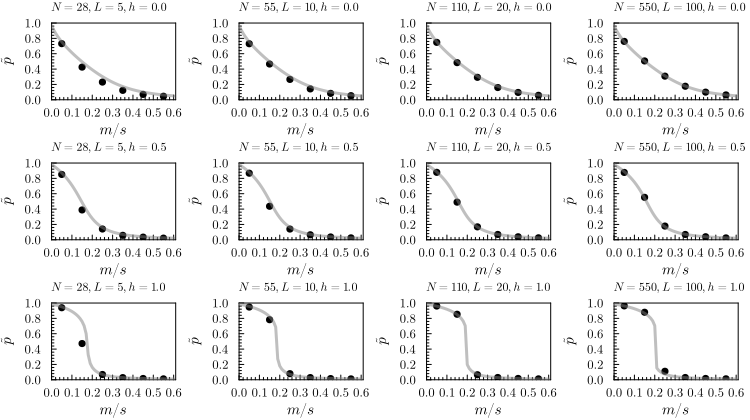
\includegraphics{/home/arthur_z/vimwiki/build/img/2023-05-03/Ls-dominance.svg}
\caption{Comparison of the multilocus diffusion approximation (gray
line) against individual-based simulations (black dots). \(Ls =1\) and
\(N_es = 5\) for all plots, while \(L\) is varied across columns
(\(L\in [5,10,25,50]\)) and \(h\) varies over rows (\(h\in[0,0.5,1]\)).
We assumed \(k=5\) diploids per haploid individual and set
\(N = N_e/2k + N_e\) so that the desired \(N_e = N_es/(Ls/L)\) is
obtained. Allele frequencies for the individual-based simulations are
obtained by simulating for 110000 generations, sampling every 5
generations after discarding the first 60000, and averaging across loci.
For each \(L\) we simulate \(n\) replicates so that \(nL = 50\). The
mutation rate was set to \(u=0.005s\).}\label{fig:Lsdom}
}
\end{figure}

\begin{figure}
\hypertarget{fig:drift}{%
\centering
\includegraphics{/home/arthur_z/vimwiki/build/img/2023-05-03/domdrift.svg}
\caption{Effect of drift on equilibrium differentiation and swamping
thresholds for a range of dominance values \(h\), ranging from
overdominant local adaptation \(h=-1\) (hybrids have an advantage), to
underdominant local adaptation \(h=2\) (hybrids perform worse than
mainland individuals on the island). All results use
\(L=40, Ls=0.8, k=5\).}\label{fig:drift}
}
\end{figure}

\begin{figure}
\hypertarget{fig:drifthm1}{%
\centering
\includegraphics{/home/arthur_z/vimwiki/build/img/2023-06-17/drift-homo-ep.svg}
\caption{Effect of genetic drift, dominance and total barrier strength
on equilibrium adaptive differentiation for a homogeneous polygenic
barrier in a diploid population. As in fig.~\ref{fig:drifthm}, but
highlighting the \(Ls\) by \(N_es\) interaction for several values of
\(m/s\).}\label{fig:drifthm1}
}
\end{figure}

\begin{figure}
\hypertarget{fig:drifthm3}{%
\centering
\includegraphics{/home/arthur_z/vimwiki/build/img/2023-06-17/drift-homo-ep2.svg}
\caption{Effect of genetic drift, dominance and total barrier strength
on equilibrium adaptive differentiation for a homogeneous polygenic
barrier in a diploid population. As in fig.~\ref{fig:drifthm}, but
highlighting the \(Ls\) by \(m/s\) interaction for several values of
\(N_es\).}\label{fig:drifthm3}
}
\end{figure}

\begin{figure}
\hypertarget{fig:hapdipeff}{%
\centering
\includegraphics{/home/arthur_z/vimwiki/build/img/2023-06-17/hapdipeff.svg}
\caption{Effective parameters accurately describe equilibrium dynamics
for haplodiplontic populations when selection is sufficiently weak. The
line shows the numerical prediction of the locally beneficial allele
frequency on the island for increasing strength of migration relative to
\emph{effective} selection. The dots show results from individual based
simulations with different degrees of haploid vs.~diploid selection and
different relative sizes of the haploid and diploid population, keeping
\(N_e, s_e\) and \(h_e\) however constant. Simulation results are based
on 110000 generations, where we sampled every 10th generation after
discarding the first 10000 generations.}\label{fig:hapdipeff}
}
\end{figure}

\begin{figure}
\hypertarget{fig:dipmig}{%
\centering
\includegraphics{/home/arthur_z/vimwiki/build/img/2023-06-30/dipmigk2.svg}
\caption{Migration in the diploid phase of a haplodiplontic life cycle
with selection in both phases leads to stronger barriers to gene flow.
The lines show predictions from the multilocus diffusion theory, whereas
the dots show results from individual-based simulations (taking a sample
every fifth generation during 20000 generations after discarding the
first 5000 generations). The migration rates in the haploid and diploid
stage are \(m_1\) and \(m_2\) respectively.}\label{fig:dipmig}
}
\end{figure}

\begin{figure}
\centering
\includegraphics[width=0.8\textwidth,height=\textheight]{/home/arthur_z/vimwiki/build/img/2023-05-04/exhet2.svg}
\caption{Predicted equilibrium allele frequencies for increasing
migration rates (left) and frequency distributions (right) for six loci
in a \(L\)-locus multilocus barrier in a diploid system, where
\(s \sim \mathrm{Exponential}(\bar{s}=0.02)\) and
\(h \sim \mathrm{Beta}(1,1)\). Lines show predictions from the
multilocus diffusion approximation, whereas dots show results from
individual-based simulations (simulating for 200000 generations after an
initial 10000, sampling every 10th generation). The frequency
distributions are shown for \(m/\bar{s} = 0.2\). \label{fig:het}}
\end{figure}

\begin{figure}
\hypertarget{fig:gffgammas}{%
\centering
\includegraphics{/home/arthur_z/vimwiki/build/img/2023-09-06/gammas-gff.svg}
\caption{The average gene flow factor across the multilocus barrier
\(\bar{g}\) for the same simulation experiment as shown in
fig.~\ref{fig:gammas}. Recall that
\(\kappa^{-1} = \mathrm{Var}[s]/\bar{s}^2\) and that \(g^{-1}\)
quantifies the strength of a barrier to gene flow.}\label{fig:gffgammas}
}
\end{figure}

\begin{figure}
\hypertarget{fig:gammash}{%
\centering
\includegraphics{/home/arthur_z/vimwiki/build/img/2023-08-10/gammas-h-notrunc.svg}
\caption{As in fig.~\ref{fig:gammas}, but where we assume
\(h_i \sim \mathrm{Beta}(1,1)\) independently for each locus in the
barrier (instead of assuming \(h_i = 1/2\) for all \(h\) as in
fig.~\ref{fig:gammas}).}\label{fig:gammash}
}
\end{figure}

\begin{figure}
\hypertarget{fig:hetfocal}{%
\centering
\includegraphics{/home/arthur_z/vimwiki/build/img/2023-08-10/hetfocal3.svg}
\caption{The effect of barrier heterogeneity on differentiation at a
focal locus. The violin plots show the distribution of \(\mathbb{E}[p]\)
at a focal locus with \(s = \bar{s}/2 = 0.0075\) (left column),
\(s=\bar{s}=0.015\) (middle column) or \(s=4\bar{s}=0.06\) (right
column) and different assumed dominance coefficients (rows) across 100
replicate simulations of a polygenic barrier with \(L\bar{s} = 1.5\) and
\(L=100\) in which this locus is embedded, for different values of
\(m/\bar{s}\) and different values of \(\kappa\), where
\(s_i \sim \mathrm{Gamma}(\kappa, \kappa/\bar{s})\) and
\(h_i \sim \mathrm{Uniform}(0,1)\) (recall that
\(\kappa^{-1} = \mathrm{Var}[s]/\bar{s}^2\)). The dots show the average
differentiation at the focal locus across the 50 replicates, whereas the
lines show \(\bar{\Delta}\), i.e.~the average expected differentiation
across the \(L\) loci in the barrier. The gray line shows the associated
single locus prediction for the focal locus. We assume \(N_es=20\) and
\(u=s/200\).}\label{fig:hetfocal}
}
\end{figure}

\begin{figure}
\hypertarget{fig:hetfocalb}{%
\centering
\includegraphics{/home/arthur_z/vimwiki/build/img/2023-08-10/hetfocal-b.svg}
\caption{The effect of barrier heterogeneity on differentiation at a
focal locus. The violin plots show the distribution of the expected
differentiation at a dominant, additive or recessive locus (from top to
bottom) with selection coefficient \(s=\bar{s}=0.015\) embedded in a
random heterogeneous barrier with
\(s_i \sim \mathrm{Gamma}(\kappa, \kappa/\bar{s})\) and
\(h_i \sim \mathrm{Uniform}(0,1)\), estimated using 100 replicate
simulations (recall that \(\kappa^{-1} = \mathrm{Var}[s]/\bar{s}^2\)).
The dots show the mean expected differentiation across replicates. The
horizontal lines show the single locus predictions for the focal locus
at the relevant value of \(m/\bar{s}\). Other parameters are as in
fig.~\ref{fig:hetfocal}.}\label{fig:hetfocalb}
}
\end{figure}

\begin{figure}
\hypertarget{fig:betas}{%
\centering
\includegraphics{/home/arthur_z/vimwiki/build/img/2023-08-10/betas-notrunc.svg}
\caption{As in fig.~\ref{fig:gammas}, but now keeping the selection
coefficient fixed at \(\bar{s} = 0.01\) and using randomly sampled
dominance coefficients, from a symmetric Beta distribution with
parameter \(\alpha\). Again,
\(L=100, N_es = 10, u/s=0.005\).}\label{fig:betas}
}
\end{figure}

\begin{figure}
\hypertarget{fig:randdiff}{%
\centering
\includegraphics{/home/arthur_z/vimwiki/build/img/2023-06-21/driftdiff.svg}
\caption{Average difference in predicted allele frequency for the single
locus vs. multilocus model. We assume \(L=100\),
\(s_i \sim \mathrm{Exponential}(\bar{s})\) and
\(h_i \sim \mathrm{Beta}(1,1)\) for \(i=1,\dots,L\). We show
\(\frac{1}{L}\sum_{i}^L |\mathbb{E}[p_{i,L}] - \mathbb{E}[p_{i,\text{single}}]|\)
where \(p_{i,L}\) and \(p_{i,\text{single}}\) are the equilibrium
frequency of the locally beneficial allele at locus \(i\) in the
multilocus model and single locus model respectively. The results are
averaged across 10 random \(L\)-locus barriers. We show results for
different strengths of genetic drift (\(N_e\bar{s}\)). Note that values
of \(L\bar{s}\) range from 0.5 to 2 (\(y\)-axis).}\label{fig:randdiff}
}
\end{figure}

\begin{figure}
\hypertarget{fig:hetscat}{%
\centering
\includegraphics{/home/arthur_z/vimwiki/build/img/2023-08-10/hetscat1.svg}
\caption{As in fig.~\ref{fig:diffdetail}, but varying the extent of
barrier heterogeneity (\(\kappa = 4,1,1/4\), rows). Results are shown
for \(L\bar{s} = 1, \bar{s}=0.01\). Recall that
\(\kappa^{-1} = \mathrm{Var}[s]/\bar{s}^2\).}\label{fig:hetscat}
}
\end{figure}

\begin{figure}
\hypertarget{fig:hetdens}{%
\centering
\includegraphics{/home/arthur_z/vimwiki/build/img/2023-08-10/hetdens1.svg}
\caption{Distributions of expected equilibrium differentiation at
individual barrier loci for the simulations shown in
fig.~\ref{fig:hetscat}.}\label{fig:hetdens}
}
\end{figure}

\begin{figure}
\hypertarget{fig:dfe1}{%
\centering
\includegraphics{/home/arthur_z/vimwiki/build/img/2023-06-25/dfe1b.svg}
\caption{As in fig.~\ref{fig:diffdetail}, but with
\(h \sim \mathrm{Beta}(2,1)\) (so that
\(\mathbb{E}[h] = 2/3\)).}\label{fig:dfe1}
}
\end{figure}

\begin{figure}
\hypertarget{fig:dfe2}{%
\centering
\includegraphics{/home/arthur_z/vimwiki/build/img/2023-06-25/dfe2b.svg}
\caption{As in fig.~\ref{fig:diffdetail}, but for the logistic
regression model (with
\(\bar{s} = 1, \kappa=1, a=7.2, b=1.2, \mathbb{E}[h] \approx 2/3, \sigma=1\);
see sec.~\ref{sec:dfe}).}\label{fig:dfe2}
}
\end{figure}

\begin{figure}
\hypertarget{fig:dfe3}{%
\centering
\includegraphics{/home/arthur_z/vimwiki/build/img/2023-06-25/dfe3b.svg}
\caption{As in fig.~\ref{fig:diffdetail}, but for the CK94 model (with
\(\bar{s}=0.01, \kappa=1\) and \(\mathbb{E}[h] = 2/3\), yielding
\(K=50\); see sec.~\ref{sec:dfe}).}\label{fig:dfe3}
}
\end{figure}

\begin{figure}
\hypertarget{fig:dfe1j}{%
\centering
\includegraphics{/home/arthur_z/vimwiki/build/img/2023-06-25/dfe1joint.svg}
\caption{Monte Carlo approximation to the joint probability distribution
of \(s\) and \(h\) conditional on observing a divergent allele on the
island (eq.~\ref{eq:msbdfe}) for the DFE model with independent
selection and dominance coefficients (see fig.~\ref{fig:diffdetail} and
sec.~\ref{sec:dfe}). Deep blue designates regions of low probability
density, bright yellow regions of high probability density. The
estimated correlation \(\rho\) between \(s\) and \(h\) is shown in the
upper right corner.}\label{fig:dfe1j}
}
\end{figure}

\begin{figure}
\hypertarget{fig:dfe1bj}{%
\centering
\includegraphics{/home/arthur_z/vimwiki/build/img/2023-06-25/dfe1bjoint.svg}
\caption{As in fig.~\ref{fig:dfe1j}, but with
\(h \sim \mathrm{Beta}(2,1)\) (see fig.~\ref{fig:dfe1} and
sec.~\ref{sec:dfe}).}\label{fig:dfe1bj}
}
\end{figure}

\begin{figure}
\hypertarget{fig:dfe2j}{%
\centering
\includegraphics{/home/arthur_z/vimwiki/build/img/2023-06-25/dfe2joint.svg}
\caption{As in fig.~\ref{fig:dfe1j}, but for the logistic model (see
fig.~\ref{fig:dfe2} and sec.~\ref{sec:dfe}).}\label{fig:dfe2j}
}
\end{figure}

\begin{figure}
\hypertarget{fig:dfe3j}{%
\centering
\includegraphics{/home/arthur_z/vimwiki/build/img/2023-06-25/dfe3joint.svg}
\caption{As in fig.~\ref{fig:dfe1j}, but for the CK94 model (see
fig.~\ref{fig:dfe3} and sec.~\ref{sec:dfe}).}\label{fig:dfe3j}
}
\end{figure}

\begin{figure}
\hypertarget{fig:dfe4}{%
\centering
\includegraphics{/home/arthur_z/vimwiki/build/img/2023-06-30/dfe4joint.svg}
\caption{As in fig.~\ref{fig:dfecomp}, but for the CK94\(^\ast\) model
with a negative correlation between \(s\) and \(h\), see
sec.~\ref{sec:dfe}. \(m/s\) values from left to right are
\(0.05, 0.20, 0.35, 0.50, 0.65\) and \(0.80\), as in
fig.~\ref{fig:dfecomp}.}\label{fig:dfe4}
}
\end{figure}

\clearpage

\hypertarget{appendix}{%
\section{Appendix}\label{appendix}}

\hypertarget{single-locus-allele-frequency-dynamics-for-weak-selection}{%
\subsection{\texorpdfstring{Single locus allele frequency dynamics for
weak selection
\label{sec:app1}}{Single locus allele frequency dynamics for weak selection }}\label{single-locus-allele-frequency-dynamics-for-weak-selection}}

Consider a single locus in a population of organisms with a
haplodiplontic life cycle. We assume a finite number \(n\) of alleles
exist at the locus. Let \(p_i\), \(i \in [0..n-1]\), denote the
frequency of the \(i\)th allele (\(A_i\)). Ignoring mutation and
migration for now, the change in allele frequency of an allele \(A_i\)
throughout the life cycle is assumed to take the form: \begin{align}
  \underbrace{
  p_i \underset{\text{haploid selection}}{\longrightarrow}
  p_i^\ast \underset{\text{gametogenesis}}{\longrightarrow}
  p_i^\ast }_{\text{haploid (gametophytic) phase}} 
  \underset{\text{syngamy}}{\longrightarrow}
  \underbrace{p_i^\ast \underset{\text{diploid selection}}{\longrightarrow}
  p_i' \underset{\text{meiosis}}
  {\longrightarrow}}_{\text{diploid (sporophytic) phase}} 
  p_i',
\end{align} where we have assumed that gametogenesis, syngamy and spore
formation do not affect the allele frequencies\footnote{Note that we use
  \(p_i^\ast\) to label the allele frequency after haploid selection,
  whereas in the main text we use this to denote the mainland allele
  frequency. Here we are not considering migration however.}. Generally,
migration could take place at any stage in the life cycle, for instance
right after meiosis (e.g.~dispersal of meiospores in bryophytes and
Fungi), at the end of the haploid phase (e.g.~gamete dispersal in
algae), early in the diploid phase (e.g.~seed dispersal in
spermatophytes) or at the level of adult diploids (e.g.~migration in
animals).

Let the relative haploid fitness of a haploid individual carrying allele
\(i\) be \(1 + \epsilon s_i\), defined as the relative contribution to
the diploid (sporophytic) generation within the haploid (gametophytic)
generation. Similarly, we let \(1+\epsilon s_{ij}\) denote the relative
fitness of a diploid individual with genotype \(A_i A_j\). The allele
frequency change over a single generation is determined by the following
dynamical system: \begin{align}
  p_i^\ast &= \frac{w_{h,i}}{\bar{w}_{h}(p)} p_i \nonumber \\
  p_i' &= \frac{w_{d,i}(p^\ast)}{\bar{w}_d(p^\ast)}p_i^\ast \qquad 1 \le i \le n,
  \label{eq:ds}
\end{align} where \(p = (p_1, p_2, \dots, p_n)\) (and similarly for
\(p^\ast\)). The marginal fitnesses \(w_{h,i}\) and \(w_{d,i}\)
associated with allele \(A_i\) in the haploid (gametophytic) and diploid
(sporophytic) phase respectively are \begin{align*}
  w_{h,i} &= 1 + \epsilon s_i \\
  w_{d,i}(p) &= \sum_j (1+\epsilon s_{ij})p_j = 1 + \epsilon\sum_j s_{ij}p_j := 1 +
  \epsilon\bar{s}_{d,i}.
\end{align*} The mean fitnesses in the gametophytic and sporophytic
phases are \begin{align*}
  \bar{w}_h(p) &= \sum_i (1+\epsilon s_i)p_i := 1 + \epsilon\bar{s}_h \\
  \bar{w}_d(p) &= \sum_i \sum_j (1+\epsilon s_{ij})p_ip_j := 1 + \epsilon\bar{s_d}
\end{align*} The allele frequency change over a single alternation of
generations for the dynamical system defined in eq.~\ref{eq:ds} has the
usual form \begin{equation}
  \Delta p_i = \frac{\bar{w}_i - \bar{w}}{\bar{w}} p_i
  \label{eq:change}
  \end{equation} Where, from eq.~\ref{eq:ds}, we have \begin{equation}
  \bar{w} = \Big(1 + \epsilon \sum_j \sum_k
  \frac{(1+\epsilon s_j)p_j (1+\epsilon s_k)p_k}{(1+\epsilon\bar{s}_h)^2} s_{jk}\Big) 
  (1+\epsilon\bar{s}_h) = 
  1 + \epsilon\bar{s}_h + \frac{\epsilon\bar{s}_s}{(1+\epsilon \bar{s}_h)^2} +
    O(\epsilon^2)
  \label{eq:wm}
\end{equation} and \[
  \bar{w_i} = \Big(1 + \epsilon
    \frac{\sum_j s_{ij}(1+\epsilon s_j)p_j}{1+\epsilon\sum_k s_k p_k}\Big)
    (1+\epsilon s_i)
  = 1 + \epsilon s_i
  + \frac{\epsilon\bar{s}_{s,i}}{(1 + \epsilon\bar{s}_h)}+
    O(\epsilon^2),
  \] so that \begin{equation}
  \bar{w_i} - \bar{w}
  = \epsilon (s_i - \bar{s}_h)
  + \frac{\epsilon}{(1 + \epsilon \bar{s}_h)^2} (\bar{s}_{d,i} - \bar{s}_d)
  + O(\epsilon^2).
  \label{eq:diff}
  \end{equation} Assuming the intensity of selection per generation is
weak (all \(s\) are small) and that \(\epsilon\) measures the generation
time, we obtain a continuous-time model of allele frequency change by
considering the per-generation change in allele frequency and taking the
limit as \(\epsilon\) goes to zero, specifically, plugging
eq.~\ref{eq:diff} and eq.~\ref{eq:wm} in eq.~\ref{eq:change}, we get
\begin{align}
  \dot{p_i} = \lim_{\epsilon\rightarrow 0}
     \frac{\Delta p_i}{\epsilon} &= 
  \big[(s_i - \bar{s}_h) + (\bar{s}_{d,i} - \bar{s}_d)\big]p_i \nonumber \\
  &= (\bar{s}_i - \bar{s})p_i,
\end{align} where \begin{align}
    \bar{s}_i &= s_i + \bar{s}_{d,i} = s_i + \sum_{j}s_{ij}p_j \nonumber \\
    \bar{s} &= \bar{s}_h + \bar{s}_{d} = \sum_i s_i p_i + \sum_i \sum_j s_{ij}
    p_i p_j.
    \label{eq:malth}
\end{align} This has the same form as the classical diploid or haploid
continuous-time model of allele frequency change\footnote{The same
  result can be obtained in a less cumbersome manner by first noting
  that, under the assumption of weak selection, allele frequency changes
  within a single alternation of generations are negligible, so that
  \(w_{s,i}(p^\ast) = w_{s,i}(p)\) and
  \(\bar{w}_s(p^\ast) = \bar{w}_s(p)\) in eq.~\ref{eq:ds}.} but with
marginal and mean Malthusian fitnesses given by \(\bar{s}_i\) and
\(\bar{s}\) respectively.

As an example, consider the biallelic case with alleles \(A_0\) and
\(A_1\), so that \(s_0 = s_{00} = 0\), \(p_0 = p\) and \(p_1=q\). Note
that we shall always assume \(s_{ij} = s_{ji}\). We have from
eq.~\ref{eq:malth} \(\bar{s}_1 = s_1 + s_{01}p + s_{11}q\) and
\(\bar{s} = s_1q + 2s_{01}pq + s_{11}q^2\). Some algebra shows that we
can write the ODE for the frequency of the selected allele (\(A_1\)) as
\begin{equation}
  \dot{q} = (\bar{s}_1 - \bar{s})q = pq(s_a + s_bq)
  \label{eq:biall}
  \end{equation} where \(s_a = s_1 + s_{01}\) and
\(s_b = s_{11} - 2s_{01}\). As expected, this is the same dynamical law
as for the strictly diploid model, in which case the dynamics of the
selected allele are given by eq.~\ref{eq:biall} but with
\(s_a = s_{01}\). This enables us to identify a pair of `effective'
selection coefficients, \begin{align}
  s_{01}^\ast = s_1 + s_{01} \nonumber \\
  s_{11}^\ast = 2s_1 + s_{11},
  \end{align} so that, for weak selection, a diploid biallelic model
with parameters \(s_{01}^\ast\) and \(s_{11}^\ast\) yields the same
allele frequency dynamics\footnote{Note that a diploid model with these
  effective parameters does \emph{not} yield the same mean fitness (and
  hence genetic load) as a haplodiplontic model in the original
  parameterization if we define mean fitness in the continuous time
  model as \(\sum_i e^{s_i} p_i \big(\sum_j e^{s_{ij}} p_j\big)\).} as a
haplodiplontic model with parameters \(s_1, s_{01}\) and \(s_{11}\).

\hypertarget{equilibrium-structure-of-the-mainland-island-model}{%
\subsection{\texorpdfstring{Equilibrium structure of the mainland-island
model
\label{sec:mieq}}{Equilibrium structure of the mainland-island model }}\label{equilibrium-structure-of-the-mainland-island-model}}

We describe the equilibrium structure of the haplodiplontic single-locus
deterministic mainland-island model for the biallelic case. The dynamics
are given by the ODE \begin{align}
    \dot{q} = - \dot{p} 
    &= m\Delta q + pq(s_a + s_b q) \label{eq:ode1} \\
    &= m\Delta q + pq(s_1 + s_{01} + (s_{11} - 2s_{01}) q),
  \end{align} where \(q\) is the frequency of the locally selected
allele \(A_1\), and \(p=1-q\) is the frequency of the allele with
relative fitness of 1 on the island when homozygous.

When \(m=0\) (no migration), there will be an admissible fixed point
when either of the following conditions holds \begin{align}
  s_{01} &> -s_1 \text{ and } s_{01} > s_1 + s_{11} \\
  s_{01} &< -s_1 \text{ and } s_{01} < s_1 + s_{11} ,
\end{align} i.e.~when there is \emph{ploidally antagonistic selection},
diploid over- or underdominance, or both. The fixed point is obtained at
\begin{equation}
  \tilde{p} = \frac{s_a + s_b}{s_a} = \frac{s_1 + s_{11} - s_{01}}{s_{11} - 2s_{01}}
  \end{equation} This will correspond to a stable polymorphism whenever
\(s_{01} > 0\). This case was first analyzed in a discrete-time model by
Scudo (1967).

Now consider \(m>0\). We shall assume that
\(\Delta q = q_{\text{mainland}} - q = 1-q = p\), i.e.~the mainland is
fixed for the locally selected allele. To describe the equilibrium
behavior, it is helpful to factor the dynamical law as \begin{equation}
  \dot{q} = mp\left(1+ \frac{s_a}{m}q + \frac{s_b}{m}q^2\right)
  \label{eq:quad}
  \end{equation} Linear stability at a fixed point \(\tilde{q}\) is
determined by \begin{align}
  \frac{d\dot{q}}{dq}\big|_{\tilde{q}} 
    &= (s_a - m) + 2(s_b-s_a)\tilde{q} -3s_b \tilde{q}^2
  \end{align} If \(s_b = 0\), we have an effectively haploid model
(i.e.~\emph{genic selection}), and will have a stable polymorphic
equilibrium at \(\tilde{q} = -m/s_a\) whenever \(m < -s_a\), and a
stable boundary equilibrium at \(\tilde{q} = 1\) when \(m > -s_a\). When
\(s_b \ne 0\), polymorphic equilibria, when they exist, will correspond
to the roots of the quadratic expression in parentheses in
eq.~\ref{eq:quad}. These are
\[q_-, q_+ = \frac{-s_a/m \pm \sqrt{(s_a/m)^2 - 4s_b/m}}{2s_b/m}\] We
have the following biologically relevant equilibria:

\begin{figure}
\centering
\includegraphics[width=0.4\textwidth,height=\textheight]{/home/arthur_z/vimwiki/build/notes/img/quadstab.pdf}
\caption{Equilibrium and stability behavior of the single-locus
biallelic haplodiplontic mainland-island model. The dark gray zone
indicates the parameter region where there is a single protected stable
polymorphic equilibrium. The light gray zone shows the parameter region
where there is both a stable (but unprotected) and an unstable
polymorphic equilibrium. \(s_1\), \(s_{01}\) and \(s_{11}\) are the
haploid and diploid selection coefficients for the invading allele
(\(A_1\)) on the island. \label{fig:stab}}
\end{figure}

\begin{enumerate}
\def\labelenumi{\roman{enumi}.}
\tightlist
\item
  \(\tilde{q}=1\) (\emph{swamping}) is always a stable equilibrium when
  \(m > -(s_a + s_b)\).
\item
  When \(0 < m < -(s_a + s_b)\) there is always a single stable
  polymorphic equilibrium at \(q_-\) (dark gray zone in
  fig.~\ref{fig:stab}) and \(q_+\) will not lie in \([0,1]\).
\item
  When \(-(s_a + s_b) < m < s_b\) and
  \(4s_b/m < (s_a/m)^2 \iff 4m < s_a^2/s_b\), there is, besides the
  stable boundary equilibrium at \(\tilde{q}=1\), an unstable
  (repelling) equilibrium at \(q_+\), and a stable polymorphic
  equilibrium at \(q_-\) (light gray zone in fig.~\ref{fig:stab}).
\end{enumerate}

The relation between the key parameters \(s_a/m\) and \(s_b/m\) and the
equilibrium behavior of the system when \(m>0\) is illustrated in
fig.~\ref{fig:stab}.

When condition (iii) holds, sharp thresholds for swamping are observed,
in which case there is a certain critical allele frequency \(p_c\) below
which no local adaptation cannot be maintained whatever the migration
rate. We can ask for which degree of dominance such sharp thresholds for
swamping can possibly be observed. From eq.~\ref{eq:quad} we see that at
an equilibrium which does not correspond to \(p=0\), the condition
\(f(q) = m + s_a q + s_bq^2 = 0\) holds. A sufficient condition for
observing a sharp threshold is that \(f\) obtains a maximum for some
\(q < 1\), hence that \(f'(1) > 0\) where \(f'(q) = s_a + 2s_bq\). This
will be the case whenever \(s_a + 2s_b > 0\). In the diploid case with
the usual parameterization where \(s_a = -sh\) and \(s_b = -s(1-2h)\),
this shows that critical behavior is expected as soon as \(h > 2/3\).

\hypertarget{sec:fp}{%
\subsection{Fixed point iteration algorithm}\label{sec:fp}}

Our approximations yield a system of equations for the expected allele
frequencies and heterozygosities on the island which are coupled through
the gff. To calculate expected allele frequencies and allele frequency
distributions at equilibrium, we solve the system self-consistently by
performing a fixed point iteration. In words: for a given initial set of
allele frequencies and heterozygosities, we calculate the gff at each
locus using eq.~\ref{eq:gff}; using these gff values, we next calculate
expected allele frequencies and heterozygosities at each locus using
numerical quadrature. This process is repeated until convergence. The
algorithm is more formally outlined in algorithm \autoref{alg:fp}.

\begin{algorithm}[t]                                                                                      
\caption{Fixed point iteration for calculating the expected allele frequency
and expected heterozygosity on the island.}\label{alg:fp}
\begin{algorithmic}[1]
\Require Initialization $p^{(0)} = (p_1^{(0)}, \dots, p_L^{(0)})$, tolerance $\epsilon$
\State $(pq)^{(0)} \leftarrow (p_1^{(0)}q_1^{(0)}, \dots, p_L^{(0)}q_L^{(0)})$
\State $n \leftarrow 1, \Delta \leftarrow \infty$
\While {$\Delta > \epsilon$}
\For{$j=1,\dots,L$}
\State $m_{e,j}^{(n)} \leftarrow \exp\left[ \sum_{i\ne j} s_{i,a} q_i^{(n-1)} +
    s_{i,b} (p_iq_i)^{(n-1)} \right]$
\State $p_j^{(n)} \leftarrow \int_0^1 p \phi(p; N_e, u, m_{e,j}^{(n)},s_j) dp$
\State $(p_jq_j)^{(n)} \leftarrow \int_0^1 p(1-p) \phi(p; N_e, u,
    m_{e,j}^{(n)},s_j) dp$
\EndFor
\State $\Delta \leftarrow \sum_j (p_j^{(n)} - p_j^{(n-1)})^2$
\State $n \leftarrow n+1$
\EndWhile
\State \Return $p^{(n)}, (pq)^{(n)}$
\end{algorithmic}
\end{algorithm}

\hypertarget{sec:supdet}{%
\subsection{Swamping thresholds for the deterministic multilocus
model}\label{sec:supdet}}

We now take a closer look at the equilibria of eq.~\ref{eq:odeq} and
their critical behavior. Clearly, \(p=0\) is always a solution of
eq.~\ref{eq:odeq}, and it will correspond to a locally stable
equilibrium (i.e.~swamping) whenever \(m/s > 1-h\). Other equilibria,
when they exist, are given by the zeros of the function \begin{equation}
  f(p) = hq + (1-2h)q^2 - \frac{m}{s}g[p] \label{eq:eq1}
\end{equation} Note that \(g[p] > 0\) and we assume \(s > 0\), so that
for any fixed \(h\), as \(m\) increases, there will indeed be a critical
migration rate beyond which \(f(p) < 0\), from which point onwards the
only stable equilibrium will be \(p=0\). At the critical point, the
equilibrium allele frequency will satisfy the additional constraint
\(f'(p) = 0\) (see fig.~\ref{fig:mlstab}), i.e. \begin{align}
  f'(p) &= h + 2(1-2h)q - 2Lm(1 - 3h - 2(1-2h)q)g[p] = 0 
  \label{eq:eq2}
  \end{align} We can solve eq.~\ref{eq:eq1} for \(g[p]\), and then plug
in \(g[p]\) in eq.~\ref{eq:eq2}. This yields a cubic polynomial in \(p\)
which can be solved for the allele frequency \(p_c\) at the critical
point: \begin{equation}
    0=Ls ((1-h)^{2}- 2p^{3} (1-2h)^2 + p^{2} (14 h^{2} - 17 h + 5) - p (7 h^{2} -
    11 h + 4)) -1 + \frac{3}{2} h + (1 - 2 h)p 
\end{equation} We can then plug \(p_c\) into eq.~\ref{eq:eq1} and solve
for \(m_c/s\). While the general expressions yield not much insight, we
can focus on a number of special cases.

Firstly, in the additive case (\(h=0.5\)), a critical point different
from \(1-h\) appears when \(Ls > 1\), in which case the equilibrium
frequency at the critical point will be \(p_c = 1-1/Ls\). The
corresponding critical migration rate is
\[\frac{m_c}{s} = \frac{e^{Ls-1}}{2Ls}.\] In the case where local
adaptation is due to dominant alleles (\(h=0\)), we have again critical
behavior as soon as \(Ls>1\), with the swamping threshold occurring at
\(m/s=1\) otherwise. In this case, we find \begin{align*}
    p_c &= \frac{3}{4} - \frac{\sqrt{L s(Ls + 8)}}{4 L s} < \frac{1}{2}, 
  & \frac{m_c}{s} = 
    \left(\frac{1}{4} + \frac{\sqrt{L s \left(L s + 8\right)}}{4Ls}\right)^{2} e^{\frac{L s}{4}
    + \frac{\sqrt{L s \left(L s + 8\right)}}{4} - 1}.
\end{align*} In contrast with the additive case (where as \(Ls\)
increases, arbitrary equilibrium differentiation can be maintained near
the critical point), equilibrium differentiation will be below \(0.5\)
near \(m_c\) when \(h=0\). Lastly, for recessive local adaptation
(\(h=1\)), we have bistable critical behavior for all \(Ls > 0\). The
equilibrium frequency at the critical point is always larger than
\(1/2\) and is given by the zeros of the cubic polynomial
\[4 Ls p^{3} - 4 Ls p^{2} + 2 p - 1 = 0\] for which we have no simple
expressions. A fair approximation for \(Ls < 1.5\) is given by
\begin{align*}
  p_c &\approx \frac{1}{2} + \frac{Ls}{4}, 
  & \frac{m_c}{s} \approx \left(\frac{1}{4} - \frac{(L s)^2}{16}  \right) 
  e^{\left(\frac{Ls}{2}\right)^{3} +  \left(\frac{L s}{\sqrt 2}\right)^2 +
    \frac{Ls}{2}}
\end{align*} The swamping threshold is seen to increase strongly with
increasing \(Ls\).

\hypertarget{sec:init}{%
\subsection{Sensitivity to initial conditions}\label{sec:init}}

\begin{figure}
\centering
\includegraphics[width=0.7\textwidth,height=\textheight]{/home/arthur_z/vimwiki/build/img/2023-04-19/example-bif-fp.svg}
\caption{Different apparent equilibria depending on initial conditions.
In the left plot, the yellow line (\(p_0 = 1\)) indicates the expected
allele frequencies as determined using the fixed point iteration of
algorithm \autoref{alg:fp}, starting with \(p^{(0)} = (1,1,\dots,1)\)
(i.e.~secondary contact, maximal initial differentiation), whereas the
green line assumes \(p^{(0)} = (0,0,\dots,0)\) (no initial
differentiation). The dots show results from individual-based
simulations with the same initial conditions (50000 generation, keeping
the last 25000 and subsampling every 5 generations). The three plots on
the right show the evolution of the fixed point iteration for different
initial initial conditions \(p^{(0)} = (p_0, p_0, \dots, p_0)\) for
three values of \(m\). Note the bifurcation of the dynamical system
defined by the algorithm: for \(m/s = 0.2\) and \(m/s=0.4\) there is a
single globally stable fixed point, whereas for \(m/s = 0.3\), there are
two locally stable fixed points. \label{fig:bifurcation}}
\end{figure}

Although the equilibrium allele frequency distribution should be
independent of the initial condition (the individual-based model can be
thought of as an ergodic Markov chain on the space of \(N\) \(L\)-locus
genotypes), for appreciable \(Ls\), the observed allele frequency
distribution in any finite-time simulation can depend strongly on the
initial conditions (that is, as \(Ls\) increases, stochastic jumps
between the different modes of the \(L\)-dimensional joint allele
frequency distribution become increasingly less likely, and occur on
time scales that are neither biologically relevant nor computationally
feasible). This is especially true in the strongly recessive case
(\(h > 2/3\)) and when LD is substantial. This is similar to the
behavior in the deterministic model: when \(Ls\) or \(h\) is
sufficiently large, and sharp swamping thresholds appear, the system is
bistable, and the polymorphic equilibrium cannot be reached when the
initial condition corresponds to a state of no or little
differentiation.

The fixed point iteration will in that case converge to an expectation
computed near one of the modes of the allele frequency distribution (see
fig.~\ref{fig:bifurcation} for an illustration). In other words,
considering the fixed point iteration outlined in algorithm
\autoref{alg:fp} as a discrete dynamical system, and treating \(m/s\) as
a bifurcation parameter, two bifurcation points occur succesively, as
shown in fig.~\ref{fig:bifurcation}. For small \(m/s\), a single
globally stable polymorphic equilibrium is obtained. After the first
bifurcation point, this equilibrium ceases to be globally stable, and a
second locally stable equilibrium corresponding to almost no
differentiation appears. After the second bifurcation point the lower
equilibrium becomes globally stable. The region of parameter space where
the two stable equilibria coexist corresponds to the situation where the
assumption of population genetic equilibrium becomes questionable, where
the state of the population after a large but finite time of evolution
depends strongly on the detailed history of the population.

\hypertarget{distribution-of-fitness-effects-dfe-models}{%
\subsection{\texorpdfstring{Distribution of fitness effects (DFE) models
\label{sec:dfe}}{Distribution of fitness effects (DFE) models }}\label{distribution-of-fitness-effects-dfe-models}}

\begin{figure}
\centering
\includegraphics[width=0.7\textwidth,height=\textheight]{/home/arthur_z/vimwiki/build/img/2023-06-22/dfejoint.svg}
\caption{Joint distributions for an example of each of the three DFE
models outlined in sec.~\ref{sec:dfe}. The joint probability density is
shown on a logarithmic scale, with yellow marking high density and
(deep) blue low density. The marginal density for the selection
coefficient is a Gamma distribution with \(\kappa = 2/3, 1, 3/2\) in the
top, middle and bottom row respectively (see sec.~\ref{sec:dfe} for the
relevant definitions). (A) Independent selection and dominance
coefficients. (B) The logistic model with \(a=9.2\) and \(b=2\). (C) The
CK94 model with \(\bar{h} = 1/3\). \label{fig:dfejoint}}
\end{figure}

\begin{figure}
\centering
\includegraphics[width=0.7\textwidth,height=\textheight]{/home/arthur_z/vimwiki/build/img/2023-06-22/dfemarg.svg}
\caption{Marginal distributions of \(s\) and \(h\) for the three example
DFE model shown in fig.~\ref{fig:dfejoint}. \label{fig:dfemarg}}
\end{figure}

\hypertarget{independent-selection-and-dominance-coefficients}{%
\subsubsection{Independent selection and dominance
coefficients}\label{independent-selection-and-dominance-coefficients}}

For the independent model, we assume, for \(i=1,\dots,L\),
\begin{align*}
    s_i &\sim \mathrm{Gamma}(\kappa, \lambda) \\
    h_i &\sim \mathrm{Beta}(\alpha, \beta),
\end{align*} where \(\kappa\) is the shape parameter of the Gamma
distribution, and \(\lambda\) the rate parameter (i.e.~the Gamma
distribution with density
\(f(s) = \Gamma(\kappa)^{-1}\lambda^{\kappa} s^{\kappa-1}e^{-\lambda s}\)).
The mean is \(\kappa/\lambda\), so that \(\lambda = \kappa/\bar{s}\).
The variance is
\(\kappa/\lambda^2 = \bar{s}^2/\kappa \propto \kappa^{-1}\) and the
excess kurtosis is similarly \(\propto \kappa^{-1}\). Decreasing
\(\kappa\) therefore increases simultaneously the variance and kurtosis
of \(s\) across the barrier. For \(\kappa = 1\), this reduces to the
Exponential distribution with rate \(\lambda\). See
fig.~\ref{fig:dfejoint} (A) and fig.~\ref{fig:dfemarg} for examples.

\hypertarget{logistic-model}{%
\subsubsection{Logistic model}\label{logistic-model}}

In the logistic model, we assume, for \(i=1,\dots,L\), \begin{align*}
    s_i &\sim \mathrm{Gamma}(\kappa, \lambda) \\
    \mathop{\mathrm{logit}}h_i |s_i &\sim \text{Normal}(a + b\log s_i,
    \sigma^2),
\end{align*} where \(\mathop{\mathrm{logit}}h = \log\frac{h}{1-h}\) is
the logit transform. In other words, we assume \(h\) to be distributed
according to a linear regression on \(\log s\) with slope \(a\) and
intercept \(b\), on a logit scale. The marginal density of \(h\) is then
\[f(h) = \frac{1}{h(1-h)}\int_0^\infty \mathrm{N}[\mathop{\mathrm{logit}}h ; a +
     b\log(s),\sigma] \mathrm{G}(s; \kappa, \lambda)ds\ ,\] where
\(\mathrm{N}(\cdot; \mu, \sigma)\) and
\(\mathrm{G}(\cdot;\kappa,\lambda)\) denote the density functions for
the Normal distribution (with mean \(\mu\) and standard deviation
\(\sigma\)) and Gamma distribution respectively. Instead of setting the
\(a\) and \(b\) parameters directly, we parameterize the regression by
choosing two reference pointst, \(s^{(1)}\) and \(s^{(2)}\), together
with their respective expected dominance coefficients
\(h^{(1)} = \mathbb{E}[h|s^{(1)}]\) and
\(h^{(2)}= \mathbb{E}[h|s^{(2)}]\) using \begin{align*}
    b &= \frac{\mathop{\mathrm{logit}}h^{(2)} - \mathop{\mathrm{logit}}h^{(1)}}{\log s^{(2)} - \log s^{(1)}} \\
    a &= \mathop{\mathrm{logit}}h^{(1)} - b\log s^{(1)}
\end{align*} This model is also illustrated in fig.~\ref{fig:dfejoint}
(B) and fig.~\ref{fig:dfemarg}.

\hypertarget{model-after-caballero1994}{%
\subsubsection{Model after Caballero and Keightley
(1994)}\label{model-after-caballero1994}}

In the model of Caballero and Keightley (1994) (see also Zhang \emph{et
al.} (2004) and discussion in Agrawal and Whitlock (2011)), referred to
as CK94, we assume \begin{align*}
    s_i &\sim \mathrm{Gamma}(\kappa, \lambda) \\
    h_i^\ast | s_i &\sim \text{Uniform}(0,e^{-Ks}) \\
    h_i &= 1 - h_i^\ast
\end{align*} It should be noted that this distribution is supposed to be
a reasonable model for dominance coefficients of deleterious mutations
at mutation-stabilizing selection equilibrium, where mutations of large
effect segregating at appreciable frequencies tend to be recessive. In
our case, we regard this as the distribution of dominance coefficients
of \emph{mutant} alleles on the \emph{mainland} that constitutes the
standing variation which is the source of locally adaptive alleles
during the initial polygenic response (which we do not explicitly
model). These are hence the dominance coefficients of the locally
\emph{beneficial} alleles on the \emph{island} (assuming dominance
coefficients to be constant across environments and genetic
backgrounds). The \(h_i\) as we defined them are however the dominance
coefficients of the invading wild-type alleles from the mainland over
the locally beneficial ones, so that we use \(h_i = 1-h_i^\ast\) where
the \(h_i^\ast\) are distributed according to the CK94 model. We set the
\(K\) parameter so that \(\mathbb{E}[h^\ast] = \bar{h}\) for some
\(\bar{h}\), i.e.
\[K =  \lambda \left((2\bar{h})^{-\frac{1}{\kappa}} - 1 \right).\] The
marginal density for \(h^\ast\) is \begin{align*}
  f(h) &= 
  \int_0^{-\frac{\log h}{K}} \frac{\lambda^\kappa}{\Gamma(\kappa)}
    \lambda^\kappa s^{\kappa-1} e^{-(\lambda - K)s} ds \\
    &= \left(\frac{\lambda}{\lambda - K}\right)^\kappa
  \int_0^{-\frac{\log h}{K}} \frac{(\lambda - K)^\kappa}{\Gamma(\kappa)}
    \lambda^\kappa s^{\kappa-1} e^{-(\lambda - K)s} ds 
    = \left(\frac{\lambda}{\lambda - K}\right)^\kappa
  \int_0^{-\frac{\log h}{K}} \mathrm{G}(s;\kappa,\lambda - K)ds \\
    &= \left(\frac{\lambda}{\lambda - K}\right)^\kappa
       \frac{\gamma\left(\kappa, -(\lambda - K) \frac{\log h}{K}\right)}{\Gamma(\kappa)}
\end{align*} where \(\gamma\) is the lower incomplete gamma function.
This model is also illustrated in fig.~\ref{fig:dfejoint} (C) and
fig.~\ref{fig:dfemarg}. To study the effect of a negative correlation
between \(s\) and \(h\) (i.e.~where strongly selected locally beneficial
alleles tend to be dominant), we use the same model, but with
\(h_i = h_i^\ast\). We refer to this model as CK94\(^\ast\) (see
fig.~\ref{fig:dfe4}).

\end{document}
